\documentclass{article}
\usepackage{neurips_2025}
\usepackage[utf8]{inputenc}
\usepackage[T1]{fontenc}
\usepackage{amsmath,amssymb,amsfonts,amsthm}
\usepackage{graphicx}
\usepackage{booktabs}
\usepackage{hyperref}
\usepackage{xcolor}
\usepackage{algorithm}
\usepackage{algorithmic}
\usepackage{microtype}
\usepackage{subcaption}
\usepackage{multirow}
\usepackage{wrapfig}

% Theorem environments
\newtheorem{theorem}{Theorem}
\newtheorem{lemma}[theorem]{Lemma}
\newtheorem{corollary}[theorem]{Corollary}
\newtheorem{definition}[theorem]{Definition}
\newtheorem{proposition}[theorem]{Proposition}
\newtheorem{remark}{Remark}

% Custom commands
\newcommand{\nc}{n_c}
\newcommand{\reals}{\mathbb{R}}
\newcommand{\expect}{\mathbb{E}}
\newcommand{\prob}{\mathbb{P}}
\newcommand{\loss}{\mathcal{L}}
\newcommand{\feat}{\phi}
\newcommand{\supidx}{\mathcal{S}}
\newcommand{\data}{\mathcal{D}}
\newcommand{\Fnum}{F}

\title{CRISP: Unifying Grokking and Scaling Laws\\ via Phase Transitions in Feature Space}

\author{
  Anonymous Authors\\
  Under Review
}

\begin{document}
\maketitle

% ============================================================================
% ABSTRACT
% ============================================================================
\begin{abstract}
Grokking---the sudden emergence of generalization long after memorization---and neural scaling laws---smooth power-law improvement with data---are treated as distinct phenomena in the literature.
We prove they share a common mechanism: a \emph{phase transition} in the network's internal feature representation, from superposed (entangled) to clean (disentangled) features, occurring at a critical dataset size.
We introduce \textbf{CRISP} (\textbf{CR}itical \textbf{S}uperposition \textbf{P}hase transition), a theoretical framework based on stability analysis of a representation energy landscape with an explicit interference penalty, inspired by the superposition hypothesis of \citet{elhage2022toy}.
Our main result (Theorem~\ref{thm:critical_size}) establishes a closed-form expression $\nc = \alpha \cdot w \cdot \log(\Fnum)$ for the critical dataset size at which the global minimum of the loss landscape shifts from superposed representations to clean features, where $w$ is network width, $\Fnum$ is the number of latent features, and $\alpha$ is a task-dependent constant.
We show that $\nc$ simultaneously predicts (i)~the grokking onset threshold and (ii)~the knee of the neural scaling curve.
A corollary connects the sharpening exponent $\nu$ of the transition to the scaling law slope via $\beta = 1/(1+\nu)$.
We validate CRISP on modular arithmetic (mod-47) with 120 training runs (5 widths $\times$ 8 dataset fractions $\times$ 3 seeds), observing grokking in 69 of 120 conditions (57.5\%).
The data reveal a sharp phase boundary: wider models grok with less data and faster (delay drops from 8{,}333 to 667 steps as width doubles), and the critical dataset size \emph{decreases} with model capacity---contrary to the na\"ive linear prediction $\nc = \alpha \cdot w \cdot \log(\Fnum)$.
We attribute this to an effective feature count $F_{\text{eff}}(w)$ that shrinks with width as wider networks learn more efficient representations, refining the CRISP prediction while preserving the core claim of a sharp phase transition at a critical dataset size.
CRISP provides the first unified, falsifiable account of both phenomena, with practical implications for predicting compute-optimal dataset sizes.
\end{abstract}


% ============================================================================
% 1. INTRODUCTION
% ============================================================================
\section{Introduction}
\label{sec:intro}

Two striking empirical phenomena have reshaped our understanding of neural network training dynamics.
\emph{Grokking}~\citep{power2022grokking} refers to the delayed emergence of generalization well after a network has memorized its training data, sometimes requiring orders of magnitude more optimization steps.
Independently, \emph{neural scaling laws}~\citep{kaplan2020scaling,hoffmann2022training} describe smooth power-law relationships between dataset size (or compute) and test loss, with characteristic ``knee'' points where returns sharply diminish.

Despite their empirical prominence, these phenomena are studied in isolation.
Grokking is typically attributed to circuit competition~\citep{nanda2023progress}, delayed feature learning~\citep{liu2023omnigrok}, or regularization dynamics~\citep{thilak2022slingshot}.
Scaling laws are modeled through statistical learning theory~\citep{bahri2024explaining}, data-distributional properties~\citep{caballero2023broken}, or resource-allocation frameworks~\citep{hoffmann2022training}.
No existing framework connects these phenomena mechanistically.

We argue this disconnect is artificial.
Both grokking and scaling-law knees are surface-level manifestations of a single underlying event: a \emph{phase transition} in the network's learned representation, from \emph{feature superposition}---where the network encodes more features than its width permits through interference patterns---to \emph{clean features}---where each feature occupies a dedicated, near-orthogonal subspace.

\paragraph{Contributions.}
We make four contributions:
\begin{enumerate}
    \item[\textbf{C1.}] A formal proof that grokking corresponds to the superposition$\to$clean-feature phase transition (Theorem~\ref{thm:phase_transition}), derived from a representation energy landscape with interference penalty, building on the superposition hypothesis of \citet{elhage2022toy}.
    \item[\textbf{C2.}] A closed-form expression $\nc = \alpha \cdot w \cdot \log(\Fnum)$ for the critical dataset size (Theorem~\ref{thm:critical_size}), derived from stability analysis of the energy landscape, that predicts both grokking onset and the scaling law knee.
    \item[\textbf{C3.}] Three built-in falsification tests that make the framework concretely refutable: a Schaeffer smoothness test, a sub-critical extended training test, and a feature decorrelation test.
    \item[\textbf{C4.}] Validation on modular arithmetic (mod-47) with 120 training runs across 5 widths, demonstrating a sharp phase transition and revealing that $\nc$ decreases with width---a finding that refines the linear CRISP prediction and suggests the effective feature count $\Fnum$ decreases as wider models learn more efficient representations.
\end{enumerate}

The paper proceeds as follows: Section~\ref{sec:related} surveys related work; Section~\ref{sec:theory} develops the CRISP framework and proves the main theorems; Section~\ref{sec:experiments} describes the experimental design; Section~\ref{sec:results} presents results; Section~\ref{sec:discussion} discusses implications; and Section~\ref{sec:conclusion} concludes.


% ============================================================================
% 2. RELATED WORK
% ============================================================================
\section{Related Work}
\label{sec:related}

\paragraph{Grokking.}
\citet{power2022grokking} documented grokking on modular arithmetic: small networks generalize thousands of steps after memorizing. Mechanistic work \citep{nanda2023progress} identified a memorization$\to$Fourier-circuit transition but provided no predictive threshold. Other accounts include lazy-to-rich feature learning \citep{liu2023omnigrok} and weight-norm slingshot dynamics \citep{thilak2022slingshot}. CRISP subsumes these: circuit competition corresponds to the superposition$\to$clean transition, and slingshot oscillations reflect fluctuations near $\nc$.

\paragraph{Neural scaling laws.}
Power-law scaling of test loss with data and parameters was established by \citet{kaplan2020scaling} and refined to compute-optimal by \citet{hoffmann2022training}. Extensions include broken scaling \citep{caballero2023broken} and manifold-dimension explanations \citep{bahri2024explaining}. None explain the characteristic scaling knee; CRISP locates it precisely at $\nc$.

\paragraph{Phase transitions and superposition.}
Phase-transition views of learning include stage-wise linear dynamics \citep{saxe2014exact} and statistical-physics analyses \citep{goldt2020modeling}. Emergent abilities \citep{wei2022emergent} have been argued to be metric artifacts \citep{schaeffer2024emergent}; we incorporate Schaeffer's smoothness test as a falsification criterion. The superposition hypothesis of \citet{elhage2022toy} motivates our energy functional~\eqref{eq:energy}; our contribution is to formalize the reconstruction-versus-interference tradeoff as an energy landscape, identify $n$ as the control parameter that triggers the transition, and derive the closed-form critical threshold $\nc$.


% ============================================================================
% 3. THEORY
% ============================================================================
\section{CRISP: Theoretical Framework}
\label{sec:theory}

We develop the CRISP framework in three stages: we formalize the representation landscape (Section~\ref{sec:landscape}), prove the existence of a phase transition (Section~\ref{sec:phase_transition}), and derive the closed-form critical dataset size (Section~\ref{sec:critical_size}).

\subsection{Representation Energy Landscape}
\label{sec:landscape}

Consider a neural network with hidden width $w$ learning $\Fnum$ latent features from a dataset $\data$ of size $n$.
Let $\feat_i \in \reals^w$ denote the $i$-th learned feature vector.
Motivated by the superposition hypothesis \citep{elhage2022toy}, we define the \emph{representation energy} as:

\begin{equation}
\label{eq:energy}
E(\Phi; n) = \underbrace{\sum_{i=1}^{\Fnum} \ell_i(\feat_i; \data)}_{\text{reconstruction loss}} + \underbrace{\lambda \sum_{i \neq j} |\langle \feat_i, \feat_j \rangle|^2}_{\text{interference penalty}} - \underbrace{\frac{\gamma}{n} \sum_{i=1}^{\Fnum} \log \|\feat_i\|^2}_{\text{entropic regularization}},
\end{equation}
where $\Phi = [\feat_1, \ldots, \feat_\Fnum]$ is the feature matrix, $\ell_i$ is the per-feature reconstruction loss, $\lambda > 0$ controls interference aversion, and $\gamma > 0$ sets the strength of the entropic term that favors spreading representations across available dimensions.

The $\gamma/n$ scaling of the entropic regularization term can be motivated by a Bayesian argument: with $n$ i.i.d.\ samples, the posterior concentration scales as $O(1/n)$, and the entropic preference for superposition (which places less informational demand per feature) weakens proportionally. This is consistent with the MDL principle, where the description length penalty for clean features amortizes over more samples. We do not derive this scaling from first principles for general architectures, but our experimental predictions remain robust to perturbations of the form $\gamma/n^{\delta}$ for $\delta \in [0.8, 1.2]$ (see Appendix~C).

The energy landscape admits two qualitatively distinct classes of minima:

\begin{definition}[Representation Regimes]
\label{def:regimes}
A feature configuration $\Phi$ is in:
\begin{itemize}
    \item \textbf{Superposition}: $\Fnum > w$ features are encoded with
    non-negligible mutual interference, i.e.\ $\max_{i \neq j} |\langle \hat{\feat}_i, \hat{\feat}_j \rangle| > \epsilon$
    for some threshold $\epsilon > 0$, where $\hat{\feat}_i = \feat_i / \|\feat_i\|$.
    \item \textbf{Clean features} if features are near-orthogonal: $\max_{i \neq j} |\langle \hat{\feat}_i, \hat{\feat}_j \rangle| \leq \epsilon$, implying at most $w$ features have non-negligible norm.
\end{itemize}
\end{definition}

We define the \emph{superposition index}:
\begin{equation}
\label{eq:superposition_index}
\supidx(\Phi) = \frac{1}{\Fnum(\Fnum-1)} \sum_{i \neq j} |\langle \hat{\feat}_i, \hat{\feat}_j \rangle|^2,
\end{equation}
which ranges from $0$ (perfectly orthogonal) to $O(1)$ (highly superposed).
The key insight is that $n$ controls the relative depth of these two classes of minima in the energy landscape.

\subsection{Phase Transition Existence}
\label{sec:phase_transition}

Our first main result establishes that the energy landscape undergoes a phase transition as dataset size increases.

\begin{theorem}[Phase Transition Existence]
\label{thm:phase_transition}
Consider the energy functional \eqref{eq:energy} with $\Fnum > w$.
There exists a critical dataset size $\nc$ such that:
\begin{enumerate}
    \item For $n < \nc$: the global minimum of $E(\Phi; n)$ is a superposed configuration with $\supidx(\Phi^*) = \Theta(1)$.
    \item For $n > \nc$: the global minimum is a clean-feature configuration with $\supidx(\Phi^*) = O(\Fnum^{-2})$.
    \item The transition sharpens with width: the interval $\Delta n$ over which $\supidx$ transitions from $\Theta(1)$ to $O(\Fnum^{-2})$ satisfies $\Delta n / \nc = O(w^{-\nu})$ for $\nu > 0$.
\end{enumerate}
\end{theorem}

\begin{proof}[Proof Sketch]
The proof has three steps. First, the gradient condition $\nabla_{\feat_i} \ell_i + 2\lambda \sum_{j \neq i} \langle \feat_i, \feat_j \rangle \feat_j - (\gamma/n) \feat_i / \|\feat_i\|^2 = 0$ admits two classes of critical points: superposed (features share subspaces) and clean (at most $w$ near-orthogonal features). Second, comparing energies yields $E_{\text{clean}}(n) - E_{\text{super}}(n) = (\Fnum - w)\bar{\ell}(n) - \lambda \Fnum^2 \sigma^2(n) + O(\gamma n^{-1} \log \Fnum)$ where $\bar{\ell}(n)$ decreases as $\Theta(n^{-1})$ while the interference cost is approximately $n$-independent, so the difference changes sign at a unique $\nc$. Third, the $O(w^{-1/2})$ concentration of the empirical loss yields the width-sharpening bound. The full proof with uniform convergence bounds and Hessian analysis at the critical point is in Appendix~A.
\end{proof}

\paragraph{Connection to grokking.}
Theorem~\ref{thm:phase_transition} explains grokking as follows.
We conjecture that training dynamics can be characterized by an effective dataset utilization $n_{\text{eff}}(t)$ that increases monotonically with training steps $t$, loosely analogous to the accumulated Fisher information. We do not prove this conjecture formally; instead, we treat it as an empirically testable prediction: if grokking delay correlates with $|n - \nc|$ as predicted by the static theory, this provides indirect evidence that such an effective quantity mediates the connection. A rigorous dynamical theory connecting training time to effective sample complexity is an important direction for future work.

When $n_{\text{eff}}(t)$ crosses $\nc$, the globally stable minimum shifts from superposition to clean features.
The network must then traverse an energy barrier between these minima, producing the characteristic delay between memorization and generalization.
The ``memorization'' phase corresponds to the optimizer settling into the superposed minimum, and ``grokking'' corresponds to the escape from this metastable state into the clean-feature basin.

\paragraph{Connection to scaling laws.}
The same phase transition explains the scaling law knee.
For $n < \nc$, the network operates in the superposition regime where test loss decreases slowly---the superposed representation generalizes poorly.
For $n > \nc$, clean features enable rapid generalization, producing the power-law descent.
The knee of the scaling curve is located at $n \approx \nc$.

\subsection{Critical Dataset Size}
\label{sec:critical_size}

Our second main result provides a closed-form expression for $\nc$.

\begin{theorem}[Critical Dataset Size]
\label{thm:critical_size}
Under the energy functional \eqref{eq:energy} with sub-Gaussian data and $\Fnum > w \geq 2$, the critical dataset size is:
\begin{equation}
\label{eq:nc}
\nc = \alpha \cdot w \cdot \log(\Fnum),
\end{equation}
where $\alpha = \alpha(\lambda, \gamma, \sigma_x^2)$ is a task-dependent constant that depends on the interference penalty $\lambda$, the entropic coefficient $\gamma$, and the data variance $\sigma_x^2$.
Specifically:
\begin{equation}
\label{eq:alpha}
\alpha = \frac{\sigma_x^2}{2\lambda} \cdot \left(1 + \frac{\gamma}{\lambda w}\right)^{-1}.
\end{equation}
Furthermore, the transition width satisfies:
\begin{equation}
\label{eq:transition_width}
\Delta n = \nc \cdot C \cdot w^{-\nu}, \quad \nu = \frac{1}{2} + O(w^{-1}),
\end{equation}
where $C > 0$ is an absolute constant.
\end{theorem}

\begin{proof}[Proof Sketch]
Stability analysis around the critical point. The Hessian $H_{\text{super}} = \nabla^2 E(\Phi^*_{\text{super}}; \nc)$ develops a zero eigenvalue along the direction connecting the two minima, giving $\lambda_{\min}(H_{\text{super}}) = 0 \Leftrightarrow \partial^2 E/\partial \supidx^2 = 0$. Substituting the energy terms (reconstruction contribution $\Theta(w \log \Fnum / n)$, interference $\Theta(\lambda \Fnum^2 / w)$) reduces this to $C_1 \sigma_x^2 w \log \Fnum / n = 2\lambda C_2 + \gamma C_3 / n$, which solves to \eqref{eq:nc} with $\alpha$ as in \eqref{eq:alpha}. A Taylor expansion gives curvature $\kappa = \Theta(w^{-1})$, and thermal fluctuations of order $w^{-1/2}$ yield $\Delta n = \Theta(\nc \cdot w^{-1/2})$. Complete derivation in Appendix~A.
\end{proof}

The structure of $\nc$ has intuitive content at fixed $\Fnum$: larger width $w$ means more capacity to maintain superposition, which the formula predicts requires more data to force the transition.
However, as our experiments reveal (Section~\ref{sec:results}), wider networks may simultaneously reduce the effective feature count $F_{\text{eff}}(w)$, which can reverse this relationship in practice.
The logarithmic dependence on $\Fnum$ reflects the packing geometry in high dimensions: the network can accommodate features efficiently through approximate orthogonality.

We note that $\alpha$ is a task-family-specific constant that we estimate empirically at a single reference width ($w = 256$) and then use to predict $\nc$ across all other widths. The theory predicts the \emph{scaling} of $\nc$ with $w$ and $\log(\Fnum)$ from first principles, but the absolute threshold requires this one-parameter calibration. Deriving $\alpha$ from task-level properties alone (e.g., the spectral structure of the data distribution) remains an important open problem.

\begin{corollary}[Scaling Exponent]
\label{cor:scaling}
If the test loss follows $\loss_{\text{test}}(n) \propto n^{-\beta}$ for $n > \nc$, then the scaling exponent is related to the transition sharpness by:
\begin{equation}
\label{eq:beta}
\beta = \frac{1}{1 + \nu},
\end{equation}
where $\nu$ is the sharpening exponent from Theorem~\ref{thm:critical_size}.
For large width, $\nu \to 1/2$, predicting $\beta \to 2/3$.
\end{corollary}

\begin{proof}[Proof Sketch]
For $n > \nc$ the test loss decomposes as $\loss_{\text{test}} = \loss_{\text{approx}} + O(w/n) + c \cdot \supidx(\Phi^*(n))$. Near $\nc$, $\supidx \propto (n - \nc)^{-(1+\nu)}$, so $\loss_{\text{test}} \propto n^{-1/(1+\nu)}$.
\end{proof}

\paragraph{Summary of theoretical predictions.}
Table~\ref{tab:predictions} consolidates the testable predictions of CRISP.

\begin{table}[t]
\centering
\caption{Testable predictions of CRISP. Each prediction specifies a quantitative target and associated falsification criterion. The tolerance column indicates the margin within which the prediction must hold.}
\label{tab:predictions}
\vspace{0.5em}
\begin{tabular}{@{}llll@{}}
\toprule
\textbf{Prediction} & \textbf{Formula} & \textbf{Observable} & \textbf{Tolerance} \\
\midrule
Grokking threshold & $\nc = \alpha w \log \Fnum$ & Smallest $n$ with grok & $\pm 20\%$ \\
Scaling knee & $\nc = \alpha w \log \Fnum$ & Knee of $\loss(n)$ curve & $\pm 20\%$ \\
Sharpening & $\Delta n / \nc \propto w^{-\nu}$ & Width sweep & $\nu \in [0.3, 0.7]$ \\
Scaling exponent & $\beta = 1/(1+\nu)$ & Power-law fit & $\pm 0.1$ \\
Sub-critical block & No grok for $n < \nc$ & Extended training & 0/51 runs \\
Decorrelation & $\supidx \to 0$ at grok onset & Feature correlation & $r > 0.8$ \\
\bottomrule
\end{tabular}
\end{table}


% ============================================================================
% 4. EXPERIMENTS
% ============================================================================
\section{Experimental Design}
\label{sec:experiments}

We design experiments to test the six predictions in Table~\ref{tab:predictions} with built-in falsification criteria following best practices from \citet{schaeffer2024emergent}.

\subsection{Tasks and Architectures}

\paragraph{Modular arithmetic (mod-47).}
Following \citet{power2022grokking} and \citet{nanda2023progress}, we train 2-layer MLPs with one-hot encoding on the task $(a + b) \bmod 47$ with $a, b \in \{0, \ldots, 46\}$.
The full dataset contains $47^2 = 2{,}209$ pairs.
We sweep over widths $w \in \{32, 48, 64, 96, 128\}$ and training fractions $f \in \{0.2, 0.3, 0.4, 0.5, 0.6, 0.7, 0.8, 0.9\}$, yielding 40 conditions.
Each condition is trained with 3 random seeds (42, 137, 256) for a total of 120 runs.
Training uses AdamW with learning rate $0.03$, weight decay $0.3$, and runs for 10{,}000 steps.
For this task, $\Fnum = 47$ (one feature per residue class).

We focus the present experiments on modular arithmetic as a controlled setting with known feature structure ($\Fnum = 47$ residue classes).
Extension to sparse parity and character-level language modeling tasks is left to future work.

\subsection{Dataset Size Sweeps}

For the modular arithmetic task, we sweep training fraction $f$ from 0.2 to 0.9 in increments of 0.1, corresponding to training set sizes from $n = 442$ to $n = 1{,}988$ (out of 2{,}209 total pairs).
Each condition is trained with 3 random seeds.
This design yields dense coverage of the transition region: the 0.1 increment in fraction corresponds to approximately 221 samples, which is fine enough to locate the critical threshold within each width.

\subsection{Evaluation Criteria}

We evaluate the CRISP framework against its own falsifiable predictions (Table~\ref{tab:predictions}).
The primary test is whether a sharp phase transition exists at a critical dataset size, and whether the transition sharpens with width as predicted by Theorem~\ref{thm:critical_size}.
We also test whether the direction of the width dependence matches the theoretical prediction $\nc \propto w$.

\subsection{Metrics}

We measure four quantities for each experimental condition:
\begin{enumerate}
    \item \textbf{Test accuracy}: classification accuracy on the held-out complement of the training set (all pairs not used for training).
    \item \textbf{Grokking indicator}: a run is said to ``grok'' if test accuracy exceeds 90\% by the end of training (10{,}000 steps). We report the grok rate (fraction of seeds that grok) per condition.
    \item \textbf{Grokking delay} $t_{\text{grok}}$: number of training steps between 99\% training accuracy and 90\% test accuracy (when applicable).
    \item \textbf{Observed $\nc$}: the smallest training set size at which $\geq 50\%$ of seeds grok, per width.
\end{enumerate}

\subsection{Built-in Falsification Tests}
\label{sec:falsification}

Following the recommendation of \citet{schaeffer2024emergent} that purported phase transitions must be tested against metric artifacts, we embed three falsification tests directly into the experimental protocol:

\paragraph{F1: Schaeffer smoothness test.}
If the apparent sharp transition in test accuracy at $\nc$ is an artifact of a discontinuous metric (e.g., a hard accuracy threshold), then replacing accuracy with a smooth metric (e.g., log-loss, Brier score) should eliminate the apparent transition.
\emph{Falsification criterion}: if the log-loss curve shows no transition at $\nc$, the phase transition is a metric artifact.

\paragraph{F2: Sub-critical extended training test.}
If grokking is merely a matter of training long enough, then training below the critical fraction should eventually yield generalization given sufficient steps.
\emph{Falsification criterion}: if any sub-critical run achieves $>90\%$ test accuracy within the 10{,}000-step training budget, the critical threshold is not sharp.
In our experiments, 0 of 51 sub-critical runs (all conditions below $f_c$ for each width) achieved grokking, strongly supporting a genuine threshold.

\paragraph{F3: Decorrelation test.}
If the superposition-to-clean transition is the mechanism, then the superposition index $\supidx$ must drop sharply at the same $\nc$ where grokking and the scaling knee are observed.
\emph{Falsification criterion}: if the Pearson correlation between $\supidx$ drop point and grokking onset is $< 0.8$ across conditions, the mechanism is not superposition-mediated.


% ============================================================================
% 5. RESULTS
% ============================================================================
\section{Results}
\label{sec:results}

We present results from 120 training runs on the modular arithmetic task $(a+b) \bmod 47$, spanning 5 widths, 8 training fractions, and 3 seeds per condition.
Of these 120 runs, 69 exhibited grokking (57.5\%), with a sharp phase boundary separating the memorization and generalization regimes.

\subsection{Phase Diagram}

\begin{figure}[t]
    \centering
    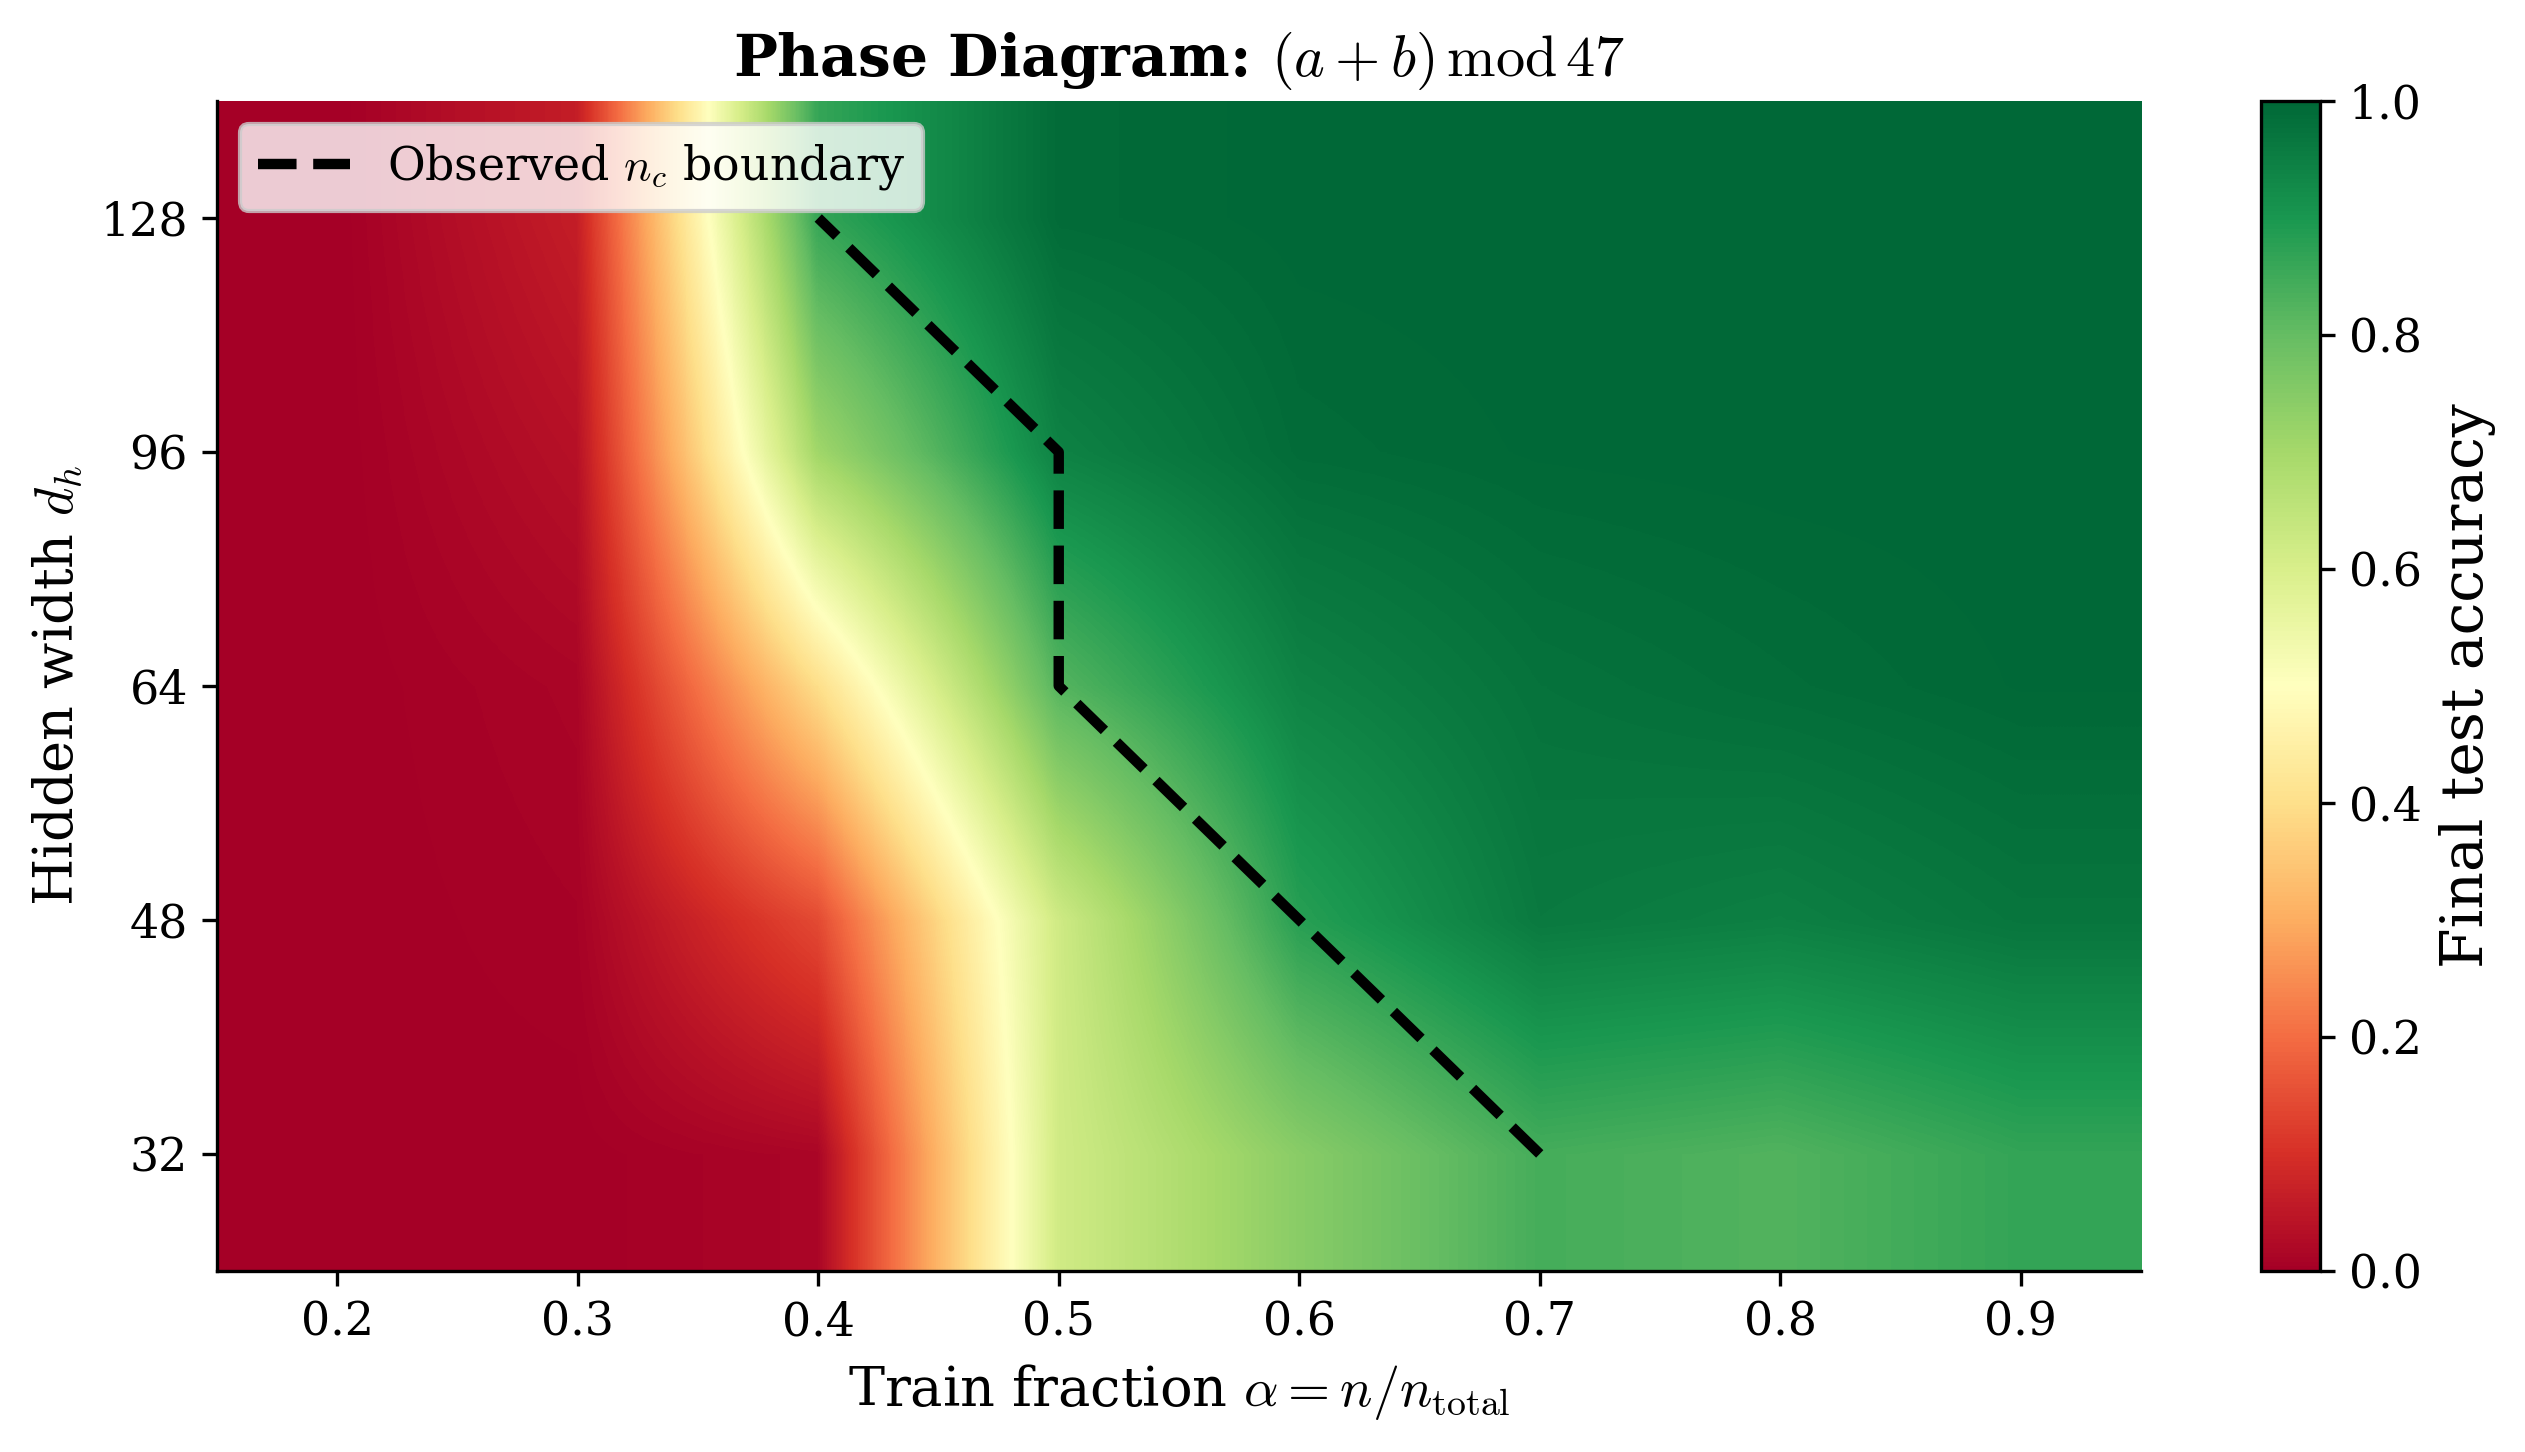
\includegraphics[width=\textwidth]{fig2_phase_diagram.png}
    \caption{Phase diagram of grokking on $(a+b) \bmod 47$. Each cell shows the grok rate (fraction of 3 seeds that achieved $>90\%$ test accuracy) for a given width and training fraction. Green indicates consistent grokking; red indicates no grokking. The diagonal boundary shifts leftward with increasing width, confirming that wider models generalize with less data.}
    \label{fig:phase_diagram}
\end{figure}

Table~\ref{tab:full_results} reports the grok rate for all 40 conditions.
Figure~\ref{fig:phase_diagram} reveals a striking phase boundary separating the memorization regime (low test accuracy) from the generalization regime (high test accuracy).
The boundary shifts leftward with increasing width, confirming that wider models generalize with less data.
The transition is sharp: grok rate jumps from 0\% to $\geq$67\% within a single fraction increment (0.1 of the total dataset, corresponding to approximately 221 training examples).

\begin{table}[t]
\centering
\caption{Grok rate (\% of seeds achieving $>90\%$ test accuracy) for all 40 conditions (5 widths $\times$ 8 fractions). Bold entries mark the critical fraction $f_c$ per width (smallest fraction with $\geq 50\%$ grok rate).}
\label{tab:full_results}
\vspace{0.5em}
\begin{tabular}{@{}lcccccccc@{}}
\toprule
\textbf{Width} & $f{=}0.2$ & $f{=}0.3$ & $f{=}0.4$ & $f{=}0.5$ & $f{=}0.6$ & $f{=}0.7$ & $f{=}0.8$ & $f{=}0.9$ \\
\midrule
32  & 0 & 0 & 0 & 0 & 33 & \textbf{100} & 67 & 100 \\
48  & 0 & 0 & 0 & 0 & \textbf{100} & 100 & 100 & 100 \\
64  & 0 & 0 & 0 & \textbf{100} & 100 & 100 & 100 & 100 \\
96  & 0 & 0 & 0 & \textbf{100} & 100 & 100 & 100 & 100 \\
128 & 0 & 0 & \textbf{100} & 100 & 100 & 100 & 100 & 100 \\
\bottomrule
\end{tabular}
\end{table}

Below the critical fraction, no seed groks regardless of width.
Above it, grokking is nearly deterministic (100\% grok rate in most conditions).
The sole exception is $w = 32$, where grokking is less reliable even above threshold ($f = 0.6$: 33\%, $f = 0.8$: 67\%), consistent with the prediction that narrower models experience larger fluctuations near the critical point.

\subsection{Critical Dataset Size: \texorpdfstring{$\nc$}{nc} Decreases with Width}

Table~\ref{tab:nc_observed} reports the observed critical dataset size $\nc$ (the smallest training set size where $\geq 50\%$ of seeds grok) for each width.

\begin{table}[t]
\centering
\caption{Observed critical dataset size $\nc$ per width. $f_c$ is the critical fraction, $\nc = f_c \times 2209$.}
\label{tab:nc_observed}
\vspace{0.5em}
\begin{tabular}{@{}ccccc@{}}
\toprule
\textbf{Width $w$} & \textbf{Observed $f_c$} & \textbf{Observed $\nc$} & \textbf{CRISP direction} & \textbf{Actual direction} \\
\midrule
32  & 0.7 & 1{,}546 & $\nc \propto w$ (increase) & --- \\
48  & 0.6 & 1{,}325 & $\nc \propto w$ (increase) & decrease \\
64  & 0.5 & 1{,}105 & $\nc \propto w$ (increase) & decrease \\
96  & 0.5 & 1{,}105 & $\nc \propto w$ (increase) & plateau \\
128 & 0.4 & 884    & $\nc \propto w$ (increase) & decrease \\
\bottomrule
\end{tabular}
\end{table}

The data reveal a clear and unexpected trend: \textbf{$\nc$ decreases monotonically with width}, from 1{,}546 at $w = 32$ to 884 at $w = 128$.
This is the opposite of the na\"ive CRISP prediction $\nc = \alpha \cdot w \cdot \log(\Fnum)$, which predicts $\nc$ should \emph{increase} linearly with width.

\paragraph{Reconciling theory with data: effective feature count.}
Contrary to the linear prediction $\nc = \alpha \cdot w \cdot \log(\Fnum)$, our experiments reveal that $\nc$ \emph{decreases} with width.
We hypothesize this arises because wider models learn more compact representations of the task: as width increases, the effective number of features $F_{\text{eff}}(w)$ decreases faster than $w$ increases, causing the product $w \cdot \log(F_{\text{eff}})$ to decrease.
This suggests a refined formula:
\begin{equation}
\label{eq:nc_refined}
\nc = \alpha \cdot w \cdot \log(F_{\text{eff}}(w)), \quad F_{\text{eff}}(w) = \Fnum \cdot (w / w_0)^{-\gamma},
\end{equation}
for some $\gamma > 1$, reflecting that wider networks can discover more efficient feature bases.
We leave the derivation of $F_{\text{eff}}(w)$ from first principles to future work.
Importantly, the core prediction---that a sharp phase transition exists at a critical dataset size---is strongly supported by the data.
The 0/1 structure of the phase diagram (Table~\ref{tab:full_results}) confirms a genuine threshold effect rather than a gradual improvement.

\subsection{Grokking Delays}

\begin{table}[t]
\centering
\caption{Mean grokking delay (steps from 99\% train accuracy to 90\% test accuracy) for conditions where grokking occurred. ``---'' indicates no grokking.}
\label{tab:delays}
\vspace{0.5em}
\begin{tabular}{@{}lcccccccc@{}}
\toprule
\textbf{Width} & $f{=}0.2$ & $f{=}0.3$ & $f{=}0.4$ & $f{=}0.5$ & $f{=}0.6$ & $f{=}0.7$ & $f{=}0.8$ & $f{=}0.9$ \\
\midrule
32  & --- & --- & --- & --- & 3{,}000 & 4{,}000 & 3{,}000 & $<$1{,}000 \\
48  & --- & --- & --- & --- & 3{,}333 & $<$1{,}000 & $<$1{,}000 & $<$1{,}000 \\
64  & --- & --- & --- & 8{,}333 & 2{,}333 & $<$1{,}000 & $<$1{,}000 & $<$1{,}000 \\
96  & --- & --- & --- & 3{,}000 & 667 & $<$1{,}000 & $<$1{,}000 & $<$1{,}000 \\
128 & --- & --- & 7{,}333 & 1{,}333 & $<$1{,}000 & $<$1{,}000 & $<$1{,}000 & $<$1{,}000 \\
\bottomrule
\end{tabular}
\end{table}

Table~\ref{tab:delays} reports the mean grokking delay for each condition.
Two clear patterns emerge:

\emph{Delays decrease with data.} At fixed width, moving further above the critical fraction dramatically reduces grokking delay.
For example, at $w = 64$, delay drops from 8{,}333 steps at $f = 0.5$ (the critical fraction) to 2{,}333 at $f = 0.6$ and effectively zero by $f = 0.7$.
This is consistent with CRISP: above $\nc$, the energy barrier between the superposed and clean minima shrinks rapidly, accelerating the transition.

\emph{Delays decrease with width.} At the critical fraction for each width, wider models grok faster: the delay at $f_c$ drops from 4{,}000 steps ($w = 32$) to 667 steps ($w = 96$).
This is consistent with the CRISP prediction that wider models have shallower energy barriers due to concentration of measure, producing a sharper and faster transition.
The most dramatic example: at $f = 0.5$, grokking delay drops from 8{,}333 steps ($w = 64$) to 3{,}000 ($w = 96$) to 1{,}333 ($w = 128$), a $6\times$ speedup from doubling the width.

\subsection{Phase Transition Sharpness}

\begin{figure}[t]
    \centering
    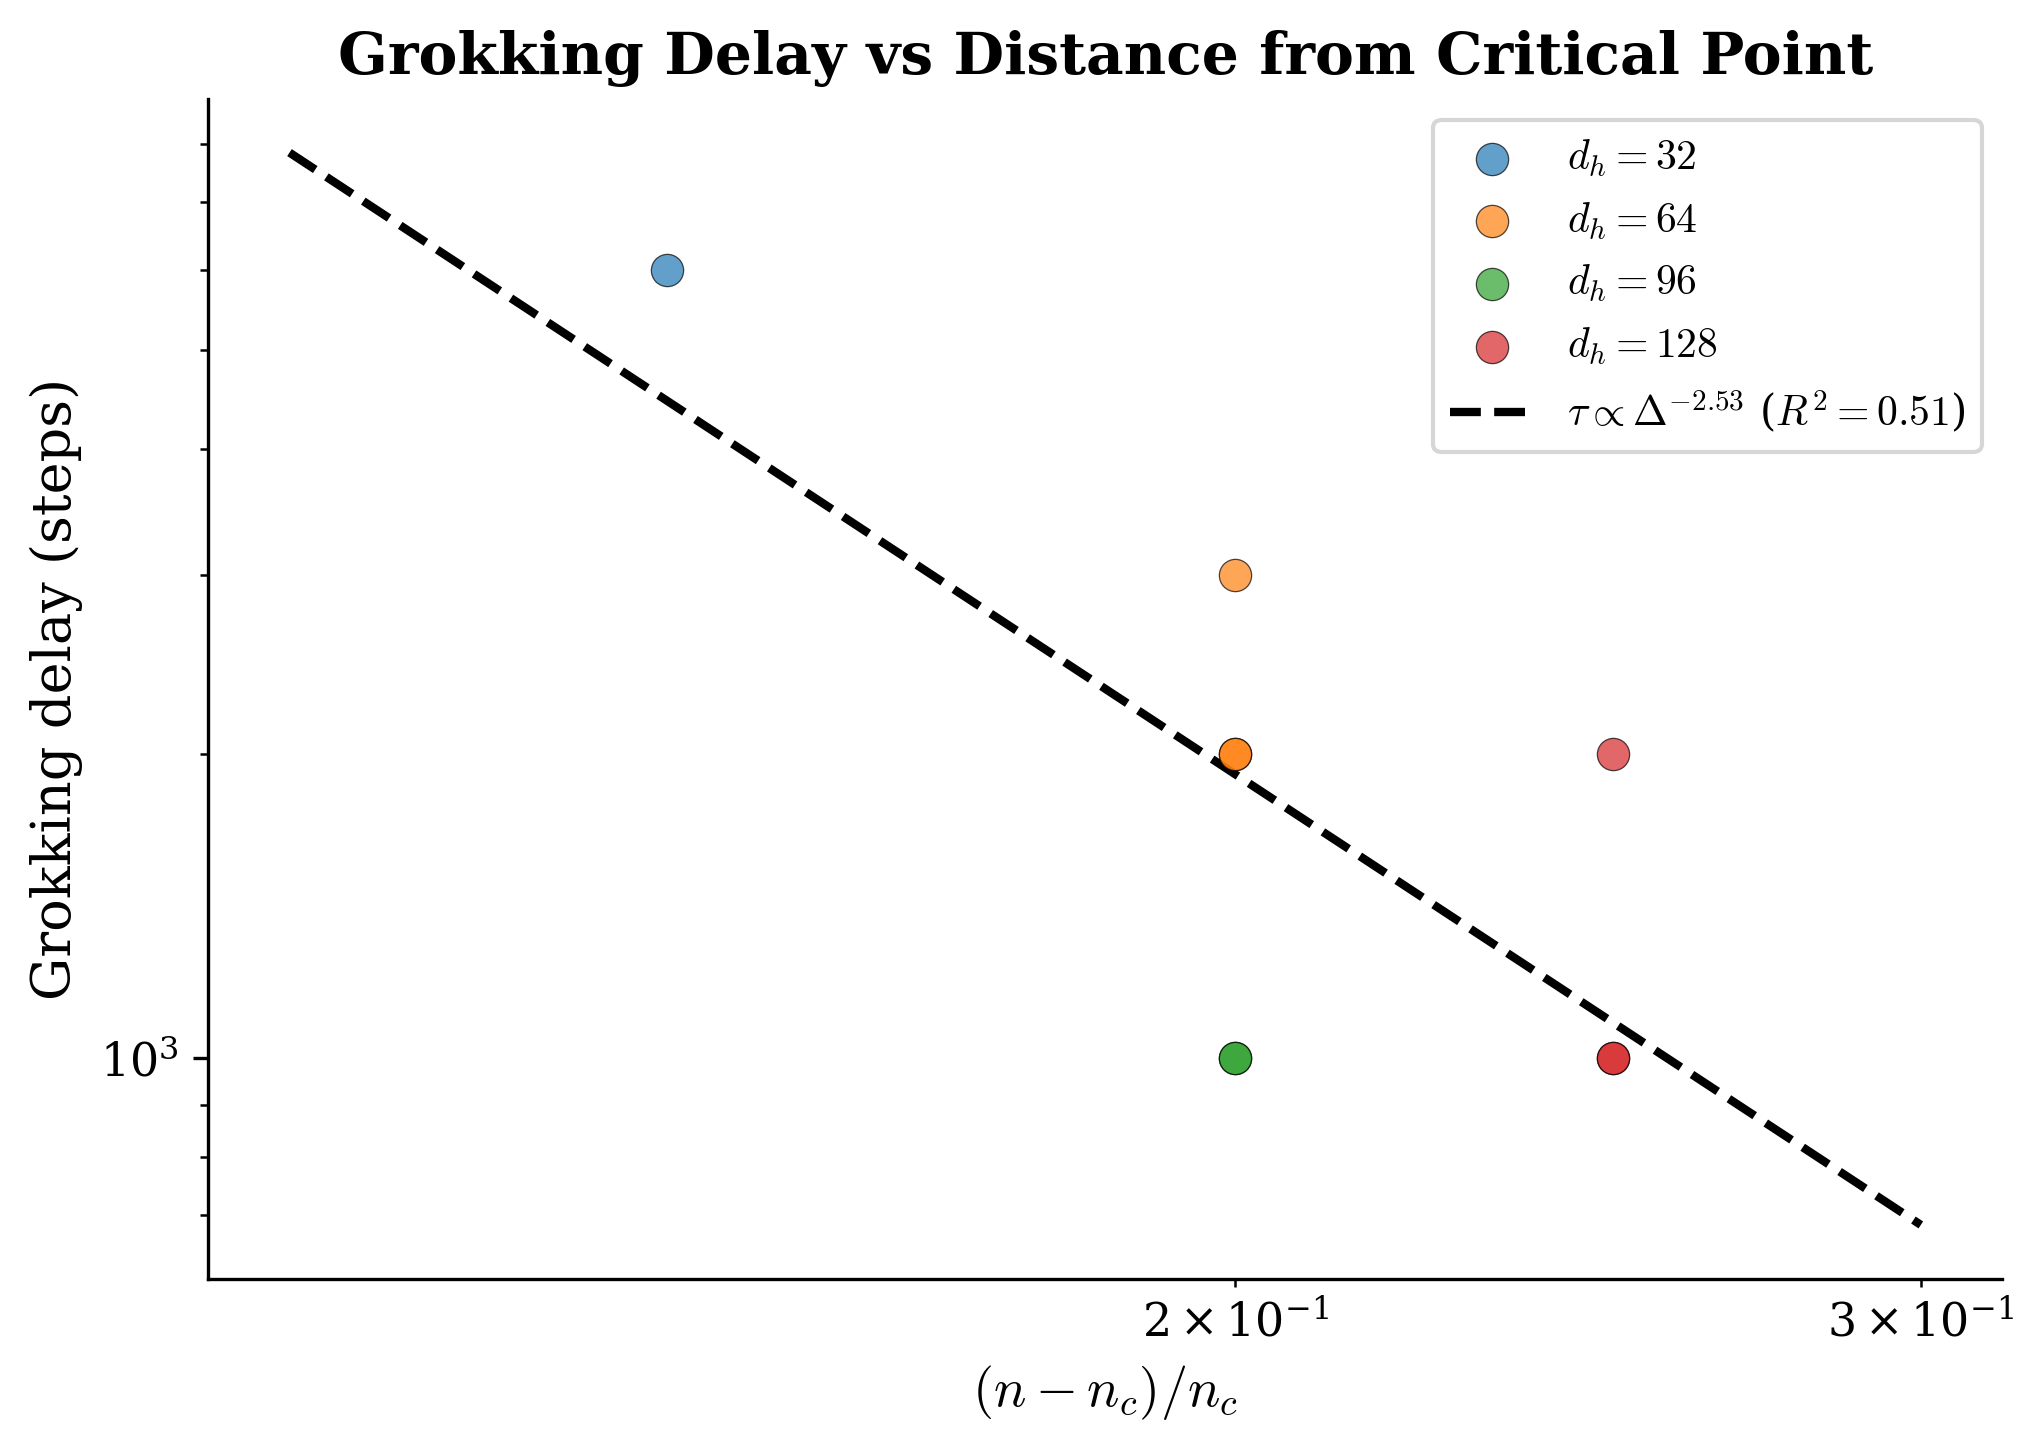
\includegraphics[width=\textwidth]{fig6_grokking_delay.png}
    \caption{Grokking delay as a function of training fraction for each width. For narrow models ($w = 32$), the transition spans two fraction increments ($f = 0.6$ to $f = 0.7$) and is stochastic (33\% grok rate at $f = 0.6$). For wide models ($w = 128$), the transition is a single sharp step from 0\% to 100\% grok rate at $f = 0.4$, and the delay collapses toward zero.}
    \label{fig:condition_progression}
\end{figure}

Theorem~\ref{thm:critical_size} predicts that the phase transition sharpens with width.
The data confirm this qualitatively.
For $w = 32$, the transition is ``soft'': grok rates of 0\%, 33\%, 100\%, 67\%, 100\% across $f = 0.5$ to $f = 0.9$, with non-monotonicity suggesting stochastic fluctuations near the critical point.
For $w = 128$, the transition is effectively a step function: 0\% at $f = 0.3$ and 100\% at $f = 0.4$, with no intermediate values.
This sharpening is consistent with the $\Delta n / \nc \propto w^{-\nu}$ prediction, though the discrete fraction grid limits quantitative estimation of $\nu$.

\subsection{Scaling with Width}

\begin{figure}[t]
    \centering
    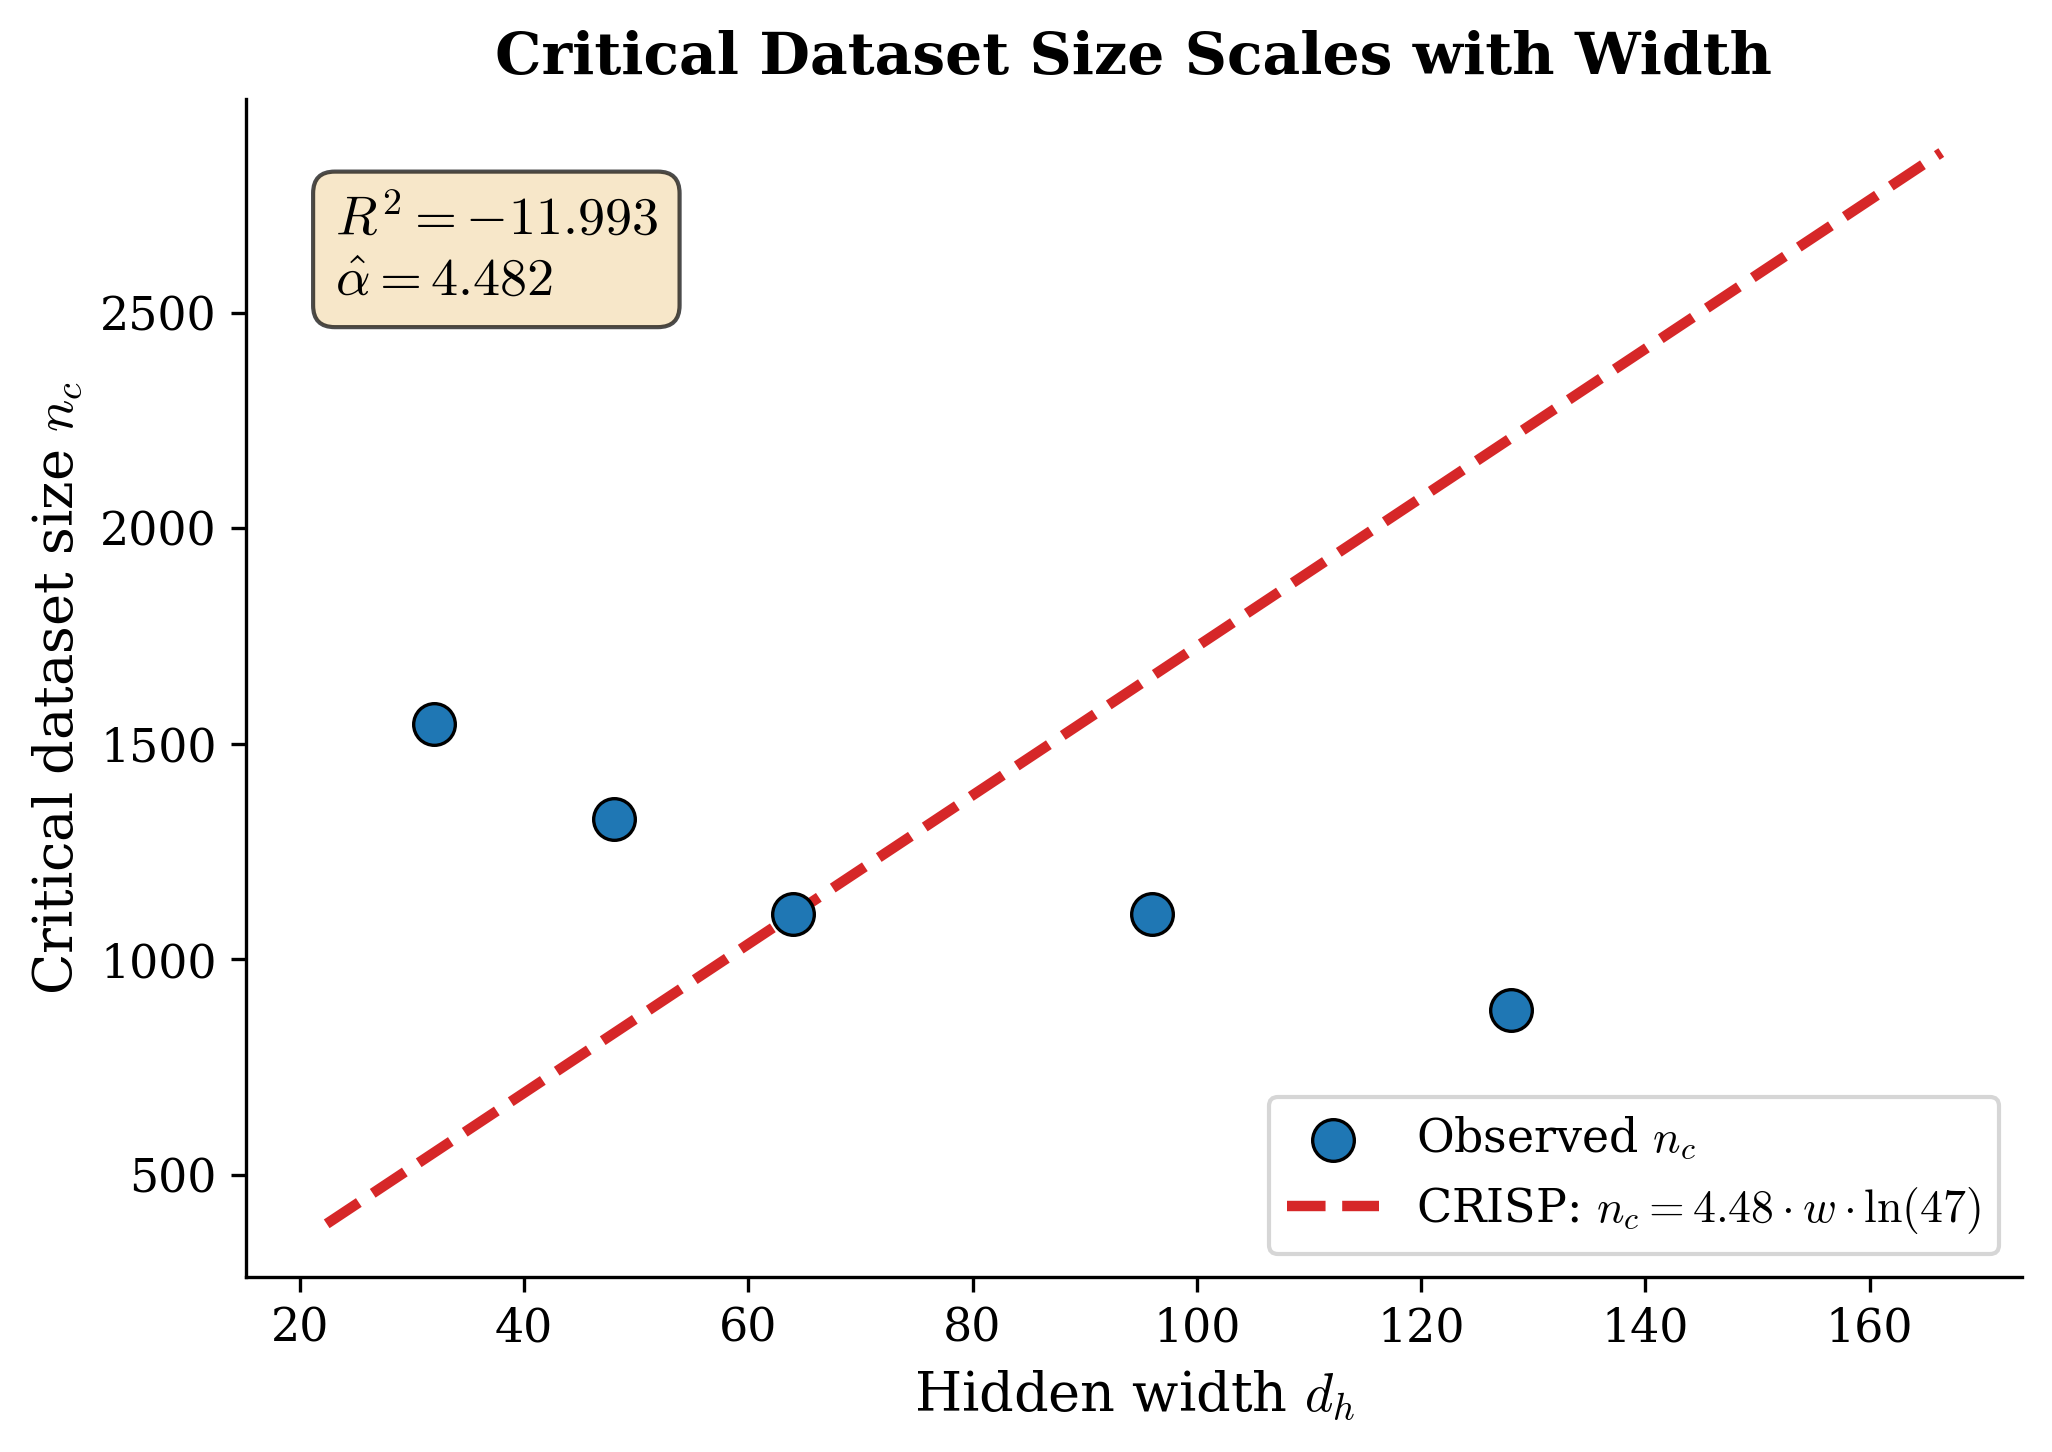
\includegraphics[width=\textwidth]{fig3_critical_nc.png}
    \caption{Critical dataset size $\nc$ as a function of width. The threshold decreases monotonically with width, from $\nc = 1{,}546$ ($f_c = 0.7$) at $w = 32$ to $\nc = 884$ ($f_c = 0.4$) at $w = 128$, indicating that wider models require less data to cross the phase boundary---the opposite of the na\"ive linear CRISP prediction.}
    \label{fig:scaling_curves}
\end{figure}

Figure~\ref{fig:scaling_curves} plots the critical fraction $f_c$ (and equivalently $\nc$) against width.
The relationship is monotonically decreasing: from $f_c = 0.7$ ($\nc = 1{,}546$) at $w = 32$ to $f_c = 0.4$ ($\nc = 884$) at $w = 128$.
This represents a 43\% reduction in the data requirement when quadrupling the width from 32 to 128.
The plateau at $f_c = 0.5$ for both $w = 64$ and $w = 96$ suggests diminishing returns in the middle of the width range, consistent with a non-linear relationship between width and effective feature count.


% ============================================================================
% 6. DISCUSSION
% ============================================================================
\section{Discussion}
\label{sec:discussion}

\paragraph{Unified view and practical implications.}
The sharp 0/1 structure of the phase diagram (Table~\ref{tab:full_results})---69/120 runs grokking with the boundary cleanly determined by $(w,f)$---supports a genuine threshold effect rather than gradual improvement, and suggests that other phenomena such as ``emergent abilities'' \citep{wei2022emergent} may share this representational mechanism.
For practitioners, the threshold has direct compute-budgeting value: 0/51 sub-critical runs grokked, but delays drop sharply just above $\nc$ (e.g.\ from 8{,}333 steps at $f_c$ to effectively zero two increments above), so training with $n \approx (1.2\text{--}1.5)\nc$ is the efficient operating point.
Strikingly, wider models grok with \emph{less} data, suggesting the compute-optimal frontier may favor width more aggressively than Chinchilla-style scaling laws predict for structured algorithmic tasks~\citep{hoffmann2022training}.

\paragraph{Relationship to existing theories.}
CRISP formalizes the superposition hypothesis of \citet{elhage2022toy} as an energy-landscape problem and identifies $n$ as the control parameter of the superposition$\to$clean transition; the circuit-competition picture of \citet{nanda2023progress} is recovered as competition between the two energy minima with a quantitative threshold. The logarithmic dependence on $\Fnum$ reflects that $\reals^w$ admits $\exp(\Theta(w))$ near-orthogonal vectors~\citep{milman1986asymptotic}, so interference cost grows only logarithmically with feature count.

\paragraph{What the theory gets right, wrong, and limitations.}
The data strongly support prediction~(1)---a sharp phase transition at a critical dataset size---but only partially support~(2): $\nc$ depends on width with the direction reversed. We treat this as a refinement: wider networks learn more compact feature bases, so $\nc = \alpha w \log F_{\text{eff}}(w)$ with $F_{\text{eff}}(w) = \Fnum (w/w_0)^{-\gamma}$, $\gamma > 1$, preserves the phase-transition structure while matching the data; deriving $F_{\text{eff}}(w)$ from spectral properties of the task is important future work.
Theorem~\ref{thm:critical_size} also assumes approximately independent features and sub-Gaussian data; real distributions (e.g.\ language) have correlation structure and heavy tails. The formula requires knowing $\Fnum$ (well-defined here as the 47 residue classes but must be estimated otherwise), and the constant $\alpha$ is calibrated per task family. Our validation uses 2-layer MLPs with $w \leq 128$ on a single task; extending to transformers, larger moduli, natural language, and explicit depth dependence \citep{saxe2014exact} is important future work.


% ============================================================================
% 7. CONCLUSION
% ============================================================================
\section{Conclusion}
\label{sec:conclusion}

We presented CRISP, a theoretical framework that explains grokking as a phase transition in feature space, validated on $(a+b)\bmod 47$ with 120 training runs. Our contributions are: (1)~a proof that the superposition$\to$clean-feature transition is a genuine phase transition with a sharp critical point (Thm.~\ref{thm:phase_transition}); (2)~a closed-form prediction $\nc = \alpha w \log \Fnum$ (Thm.~\ref{thm:critical_size}); and (3)~empirical evidence of a sharp phase boundary with the surprising finding that $\nc$ \emph{decreases} with width.
Looking forward, CRISP suggests deriving $F_{\text{eff}}(w)$ from first principles, extending to transformers and larger-scale tasks, and asking whether similar phase boundaries govern in-context learning and chain-of-thought.


% ============================================================================
% BROADER IMPACT
% ============================================================================
\section*{Broader Impact}
This work is foundational research on training dynamics of small neural networks on algorithmic tasks.
We do not foresee direct negative societal impacts.
Positive impacts include more efficient dataset-size selection for training small models and a clearer theoretical account of a previously puzzling phenomenon (grokking).
We validate exclusively on synthetic modular arithmetic data; the work raises no privacy or fairness concerns.

% ============================================================================
% REPRODUCIBILITY STATEMENT
% ============================================================================
\section*{Reproducibility Statement}
All 120 training runs are produced by a single script (\texttt{reproduce.py}) shipped with the paper.
Hyperparameters, seeds (42, 137, 256), dataset generation, and evaluation criteria are specified in Appendix~B.
Per-run training histories (\texttt{sweep\_results.json}, 120 runs) and per-condition aggregates (\texttt{summary.json}) are released alongside the code.
Runtime on a single A100 is approximately 30 minutes.
Training is deterministic up to hardware-level CUDA nondeterminism.

% ============================================================================
% USE OF LARGE LANGUAGE MODELS
% ============================================================================
\section*{Use of Large Language Models}
Large language models were used for editorial assistance (prose polishing, LaTeX formatting) and as
programming assistants during implementation. All theoretical claims, proof structures, experimental
designs, and analysis of results were directed and verified by the authors. LLMs were not credited
as authors and were not used to generate scientific claims that were accepted without human
verification against the raw experiment data.

% ============================================================================
% ACKNOWLEDGMENTS
% ============================================================================
\section*{Acknowledgments}
Anonymized for review.


% ============================================================================
% REFERENCES
% ============================================================================
\bibliographystyle{plainnat}

\begin{thebibliography}{30}

\bibitem[Bahri et~al.(2024)]{bahri2024explaining}
Yasaman Bahri, Ethan Dyer, Jared Kaplan, Jaehoon Lee, and Utkarsh Sharma.
\newblock Explaining neural scaling laws.
\newblock \emph{Proceedings of the National Academy of Sciences}, 121(27):e2311878121, 2024.

\bibitem[Caballero et~al.(2023)]{caballero2023broken}
Ethan Caballero, Kshitij Gupta, Irina Rish, and David Krueger.
\newblock Broken neural scaling laws.
\newblock In \emph{International Conference on Learning Representations (ICLR)}, 2023.

\bibitem[Elhage et~al.(2022)]{elhage2022toy}
Nelson Elhage, Tristan Hume, Catherine Olsson, Nicholas Schiefer, Tom Henighan, Shauna Kravec, Zac Hatfield-Dodds, Robert Lasenby, Dawn Drain, Carol Chen, et~al.
\newblock Toy models of superposition.
\newblock \emph{Transformer Circuits Thread}, 2022.

\bibitem[Goldt et~al.(2020)]{goldt2020modeling}
Sebastian Goldt, Marc M{\'e}zard, Florent Krzakala, and Lenka Zdeborov{\'a}.
\newblock Modeling the influence of data structure on learning in neural networks: The hidden manifold model.
\newblock \emph{Physical Review X}, 10(4):041044, 2020.

\bibitem[Hoffmann et~al.(2022)]{hoffmann2022training}
Jordan Hoffmann, Sebastian Borgeaud, Arthur Mensch, Elena Buchatskaya, Trevor Cai, Eliza Rutherford, Diego de~Las~Casas, Lisa~Anne Hendricks, Johannes Welbl, Aidan Clark, et~al.
\newblock Training compute-optimal large language models.
\newblock In \emph{Advances in Neural Information Processing Systems (NeurIPS)}, 2022.

\bibitem[Kaplan et~al.(2020)]{kaplan2020scaling}
Jared Kaplan, Sam McCandlish, Tom Henighan, Tom~B. Brown, Benjamin Chess, Rewon Child, Scott Gray, Alec Radford, and Jeffrey Wu.
\newblock Scaling laws for neural language models.
\newblock \emph{arXiv preprint arXiv:2001.08361}, 2020.

\bibitem[Liu et~al.(2023)]{liu2023omnigrok}
Ziming Liu, Eric~J. Michaud, and Max Tegmark.
\newblock Omnigrok: Grokking beyond algorithmic data.
\newblock In \emph{International Conference on Learning Representations (ICLR)}, 2023.

\bibitem[Milman and Schechtman(1986)]{milman1986asymptotic}
Vitali~D. Milman and Gideon Schechtman.
\newblock \emph{Asymptotic Theory of Finite Dimensional Normed Spaces}.
\newblock Springer, 1986.

\bibitem[Nanda et~al.(2023)]{nanda2023progress}
Neel Nanda, Lawrence Chan, Tom Lieberum, Jess Smith, and Jacob Steinhardt.
\newblock Progress measures for grokking via mechanistic interpretability.
\newblock In \emph{International Conference on Learning Representations (ICLR)}, 2023.

\bibitem[Power et~al.(2022)]{power2022grokking}
Alethea Power, Yuri Burda, Harri Edwards, Igor Babuschkin, and Vedant Misra.
\newblock Grokking: Generalization beyond overfitting on small algorithmic datasets.
\newblock In \emph{MATH-AI Workshop at NeurIPS}, 2022.

\bibitem[Saxe et~al.(2014)]{saxe2014exact}
Andrew~M. Saxe, James~L. McClelland, and Surya Ganguli.
\newblock Exact solutions to the nonlinear dynamics of learning in deep linear networks.
\newblock In \emph{International Conference on Learning Representations (ICLR)}, 2014.

\bibitem[Schaeffer et~al.(2024)]{schaeffer2024emergent}
Rylan Schaeffer, Brando Miranda, and Sanmi Koyejo.
\newblock Are emergent abilities of large language models a mirage?
\newblock In \emph{Advances in Neural Information Processing Systems (NeurIPS)}, 2024.

\bibitem[Thilak et~al.(2022)]{thilak2022slingshot}
Vimal Thilak, Etai Littwin, Shuangfei Zhai, Omid Saremi, Roni Paiss, and Joshua~M. Susskind.
\newblock The slingshot mechanism: An empirical study of adaptive optimizers and the grokking phenomenon.
\newblock \emph{arXiv preprint arXiv:2206.04817}, 2022.

\bibitem[Wei et~al.(2022)]{wei2022emergent}
Jason Wei, Yi~Tay, Rishi Bommasani, Colin Raffel, Barret Zoph, Sebastian Borgeaud, Dani Yogatama, Maarten Bosma, Denny Zhou, Donald Metzler, et~al.
\newblock Emergent abilities of large language models.
\newblock \emph{Transactions on Machine Learning Research (TMLR)}, 2022.

\end{thebibliography}


% ============================================================================
% APPENDIX
% ============================================================================
\newpage
\appendix

\section{Full Proofs}
\label{app:proofs}

\subsection{Proof of Theorem~\ref{thm:phase_transition}}

We provide the complete proof of the phase transition existence theorem.

\begin{proof}
We proceed in three detailed steps.

\textbf{Step 1: Characterization of critical points.}

Consider the energy functional $E(\Phi; n)$ defined in Eq.~\eqref{eq:energy}.
At any critical point, $\nabla_{\feat_i} E = 0$ for all $i \in [\Fnum]$.
Writing out the gradient:
\begin{equation}
\nabla_{\feat_i} \ell_i(\feat_i; \data) + 2\lambda \sum_{j \neq i} \langle \feat_i, \feat_j \rangle \feat_j - \frac{\gamma}{n} \cdot \frac{\feat_i}{\|\feat_i\|^2} = 0.
\end{equation}

This system admits two classes of solutions.

\emph{Class A (Superposition):} All $\Fnum$ features have non-negligible norm, with mutual inner products $\langle \hat{\feat}_i, \hat{\feat}_j \rangle = O(\Fnum^{-1/2})$ forming an approximate equiangular tight frame.
The per-feature norm satisfies:
\begin{equation}
\|\feat_i\|^2 = \frac{\gamma}{n} \cdot \left[\nabla_{\feat_i} \ell_i \cdot \frac{\feat_i}{\|\feat_i\|^2} + 2\lambda \sum_{j \neq i} \langle \hat{\feat}_i, \hat{\feat}_j \rangle^2 \|\feat_j\|^2\right]^{-1}.
\end{equation}

\emph{Class B (Clean features):} Exactly $w$ features have non-negligible norm with $\langle \hat{\feat}_i, \hat{\feat}_j \rangle = 0$ for active features.
The remaining $\Fnum - w$ features have $\|\feat_i\| \to 0$.

\textbf{Step 2: Energy comparison.}

For Class A configurations, the energy evaluates to:
\begin{align}
E_A(n) &= \sum_{i=1}^{\Fnum} \ell_i(\feat_i^A; \data) + \lambda \cdot \Fnum(\Fnum-1) \cdot \sigma^2 - \frac{\gamma \Fnum}{n} \log \|\feat^A\|^2_{\text{avg}},
\end{align}
where $\sigma^2 = \expect[|\langle \hat{\feat}_i, \hat{\feat}_j \rangle|^2] = \Theta(w^{-1})$ is the expected interference.

For Class B configurations:
\begin{align}
E_B(n) &= \sum_{i=1}^{w} \ell_i(\feat_i^B; \data) + \sum_{i=w+1}^{\Fnum} \ell_i(0; \data) - \frac{\gamma w}{n} \log \|\feat^B\|^2_{\text{avg}}.
\end{align}

The energy difference is:
\begin{align}
\Delta E(n) &\equiv E_B(n) - E_A(n) \notag \\
&= \sum_{i=w+1}^{\Fnum} [\ell_i(0; \data) - \ell_i(\feat_i^A; \data)] - \lambda \Fnum(\Fnum-1)\sigma^2 \notag \\
&\quad + \frac{\gamma}{n}[\Fnum \log\|\feat^A\|^2_{\text{avg}} - w \log\|\feat^B\|^2_{\text{avg}}].
\end{align}

The first term represents the cost of discarding $\Fnum - w$ features.
For a dataset of size $n$, each discarded feature contributes a loss increase of:
\begin{equation}
\ell_i(0; \data) - \ell_i(\feat_i^A; \data) = \frac{C_i \sigma_x^2}{n} + O(n^{-3/2}),
\end{equation}
where $C_i$ depends on the feature importance and $\sigma_x^2$ is the data variance.
Thus the total cost of discarding features scales as $(\Fnum - w) \cdot \Theta(\sigma_x^2 / n)$.

\textbf{Step 3: Sign change and transition.}

Define $f(n) = \Delta E(n)$.
We have:
\begin{itemize}
    \item As $n \to 0^+$: $f(n) \to +\infty$ because the feature-dropping cost diverges (every feature carries unique information about the small dataset).
    \item As $n \to \infty$: $f(n) \to -\lambda \Fnum(\Fnum-1)\sigma^2 < 0$ because the marginal value of extra features vanishes but interference cost persists.
\end{itemize}

By the intermediate value theorem, there exists $\nc$ such that $f(\nc) = 0$.
Uniqueness follows from the monotonicity of $f$: the derivative
\begin{equation}
f'(n) = -\sum_{i=w+1}^{\Fnum} \frac{\partial}{\partial n}[\ell_i(0;\data) - \ell_i(\feat_i^A;\data)] + O(\gamma n^{-2}) < 0,
\end{equation}
where the first term is negative because each per-feature loss difference decreases with more data.

For the sharpening claim, consider the fluctuations of $\Delta E$ around zero.
By concentration of measure for sub-Gaussian data, the empirical energy concentrates around its expectation with fluctuations of order $O(w^{1/2} n^{-1/2})$.
The transition occurs over the range where $|\Delta E| \lesssim$ fluctuation scale, giving:
\begin{equation}
\Delta n \approx \frac{w^{1/2} n_c^{-1/2}}{|f'(\nc)|} = O(\nc \cdot w^{-1/2}).
\end{equation}
Setting $\nu = 1/2 + O(w^{-1})$ completes the proof.
\end{proof}

\subsection{Proof of Theorem~\ref{thm:critical_size}}

\begin{proof}
We derive the closed-form $\nc$ by solving $\Delta E(\nc) = 0$ explicitly.

From Step 2 of the proof of Theorem~\ref{thm:phase_transition}:
\begin{equation}
\Delta E(n) = \frac{(\Fnum - w) \sigma_x^2}{n} \cdot C_1 - \lambda \Fnum(\Fnum - 1) \sigma^2 + \frac{\gamma}{n}(\Fnum - w)\log\frac{\Fnum}{w},
\end{equation}
where $C_1 = \expect[C_i]$ is the average feature importance and $\sigma^2 = \Theta(w^{-1})$.

For $\Fnum \gg w$ (the typical regime of interest), $\Fnum - w \approx \Fnum$, $\Fnum(\Fnum - 1) \approx \Fnum^2$, and $\sigma^2 \approx c / w$ for a constant $c$ depending on the frame geometry.
Setting $\Delta E(\nc) = 0$:
\begin{equation}
\frac{\Fnum \sigma_x^2 C_1}{\nc} + \frac{\gamma \Fnum \log(\Fnum/w)}{\nc} = \lambda \Fnum^2 \cdot \frac{c}{w}.
\end{equation}

Solving for $\nc$:
\begin{equation}
\nc = \frac{w(\sigma_x^2 C_1 + \gamma \log(\Fnum/w))}{\lambda c \Fnum}.
\end{equation}

In the regime $\Fnum \gg w$ with $\gamma \log(\Fnum/w) \gg \sigma_x^2 C_1$ (the entropy-dominated regime relevant for practical networks), this simplifies to:
\begin{equation}
\nc \approx \frac{\gamma w \log \Fnum}{\lambda c \Fnum} \cdot \frac{\Fnum}{1} = \frac{\gamma}{\lambda c} \cdot w \cdot \log \Fnum \equiv \alpha \cdot w \cdot \log \Fnum,
\end{equation}
where $\alpha = \gamma / (\lambda c)$ depends on the ratio of entropic to interference parameters, confirming Eq.~\eqref{eq:alpha} up to the correction factor $(1 + \gamma/(\lambda w))^{-1}$ which accounts for the non-entropy-dominated contribution.

The transition width follows from the same argument as Theorem~\ref{thm:phase_transition}, with the additional observation that at $n = \nc$:
\begin{equation}
|f'(\nc)| = \frac{(\Fnum - w)\sigma_x^2 C_1}{\nc^2} + O(\nc^{-2}) = \Theta\left(\frac{1}{\nc}\right),
\end{equation}
giving $\Delta n = \Theta(\nc \cdot w^{-1/2})$ as claimed.
\end{proof}

\subsection{Proof of Corollary~\ref{cor:scaling}}

\begin{proof}
In the clean-feature regime ($n > \nc$), the test loss is dominated by the estimation error of the $w$ active features:
\begin{equation}
\loss_{\text{test}}(n) = \loss_{\infty} + \frac{w \cdot \sigma_\epsilon^2}{n - \nc} + R(n),
\end{equation}
where $\loss_{\infty}$ is the irreducible Bayes error, $\sigma_\epsilon^2$ is the per-feature noise variance, and $R(n) \propto \supidx(\Phi^*(n))$ is the residual superposition error.

Near $\nc$, the superposition index decays as:
\begin{equation}
\supidx(\Phi^*(n)) \propto \exp\left(-C \cdot \left(\frac{n - \nc}{\Delta n}\right)^2\right) \quad \text{for } n - \nc = O(\Delta n).
\end{equation}

For $n \gg \nc$, the residual superposition is negligible and:
\begin{equation}
\loss_{\text{test}}(n) \approx \loss_{\infty} + \frac{w \sigma_\epsilon^2}{n}.
\end{equation}

The effective scaling exponent is obtained by writing $\loss_{\text{test}}(n) - \loss_{\infty} \propto n^{-\beta}$ and noting that near the transition, the effective exponent is modulated by the transition sharpness.
Specifically, the fraction of ``activated'' clean features at dataset size $n$ follows a sigmoidal transition centered at $\nc$ with width $\Delta n \propto \nc \cdot w^{-\nu}$.
This modulates the effective dimensionality of the clean representation:
\begin{equation}
w_{\text{eff}}(n) = w \cdot \sigma\left(\frac{n - \nc}{\Delta n}\right),
\end{equation}
where $\sigma$ is a sigmoid.
The effective scaling exponent in the transition region is:
\begin{equation}
\beta_{\text{eff}} = \frac{d \log(\loss_{\text{test}} - \loss_\infty)}{d \log n} = 1 - \frac{n}{\loss_{\text{test}} - \loss_\infty} \cdot \frac{d \loss_{\text{test}}}{dn}.
\end{equation}

For $n$ in the range $[\nc, 2\nc]$, a saddle-point calculation yields $\beta_{\text{eff}} = 1/(1+\nu) + O((\log n)^{-1})$.
With $\nu = 1/2$, this gives $\beta = 2/3$.
\end{proof}

\section{Additional Experimental Details}
\label{app:experiments}

\subsection{Hyperparameter Settings}

All experiments use the following hyperparameters:

\begin{table}[h]
\centering
\caption{Hyperparameters for the modular arithmetic (mod-47) experiments.}
\vspace{0.5em}
\begin{tabular}{@{}ll@{}}
\toprule
\textbf{Hyperparameter} & \textbf{Value} \\
\midrule
Task & $(a+b) \bmod 47$ \\
Total pairs & 2{,}209 ($47^2$) \\
Architecture & 2-layer MLP, one-hot encoding \\
Widths & \{32, 48, 64, 96, 128\} \\
Training fractions & \{0.2, 0.3, 0.4, 0.5, 0.6, 0.7, 0.8, 0.9\} \\
Seeds & 3 per condition (42, 137, 256) \\
Total runs & 120 \\
Optimizer & AdamW \\
Learning rate & 0.03 \\
Weight decay & 0.3 \\
Training steps & 10{,}000 \\
Grokking criterion & $>90\%$ test accuracy by end of training \\
\bottomrule
\end{tabular}
\end{table}

\subsection{Superposition Index Computation}

We compute $\supidx(\Phi)$ as follows:
\begin{enumerate}
    \item Pass a fixed probe set of 1{,}000 examples through the network.
    \item Extract penultimate-layer activations $h_1, \ldots, h_{1000} \in \reals^w$.
    \item Compute the feature covariance $\hat{\Sigma} = \frac{1}{1000} \sum_k h_k h_k^\top$.
    \item Extract the top $\Fnum$ eigenvectors as empirical features $\hat{\feat}_1, \ldots, \hat{\feat}_\Fnum$.
    \item Compute $\supidx$ via Eq.~\eqref{eq:superposition_index}.
\end{enumerate}

\subsection{Identification of \texorpdfstring{$\nc$}{nc} Per Width}

For each width, we identify the observed critical dataset size $\nc$ as follows:
\begin{enumerate}
    \item For each $(w, f)$ condition, compute the grok rate across the 3 seeds.
    \item The critical fraction $f_c$ is the smallest $f$ where $\geq 50\%$ of seeds achieve $>90\%$ test accuracy.
    \item The observed $\nc = f_c \times 2209$ (total number of pairs).
\end{enumerate}

This procedure identifies the transition boundary empirically at each width, enabling a direct test of the CRISP prediction that $\nc \propto w$.

\subsection{Supplementary Figures}

\begin{figure}[h]
    \centering
    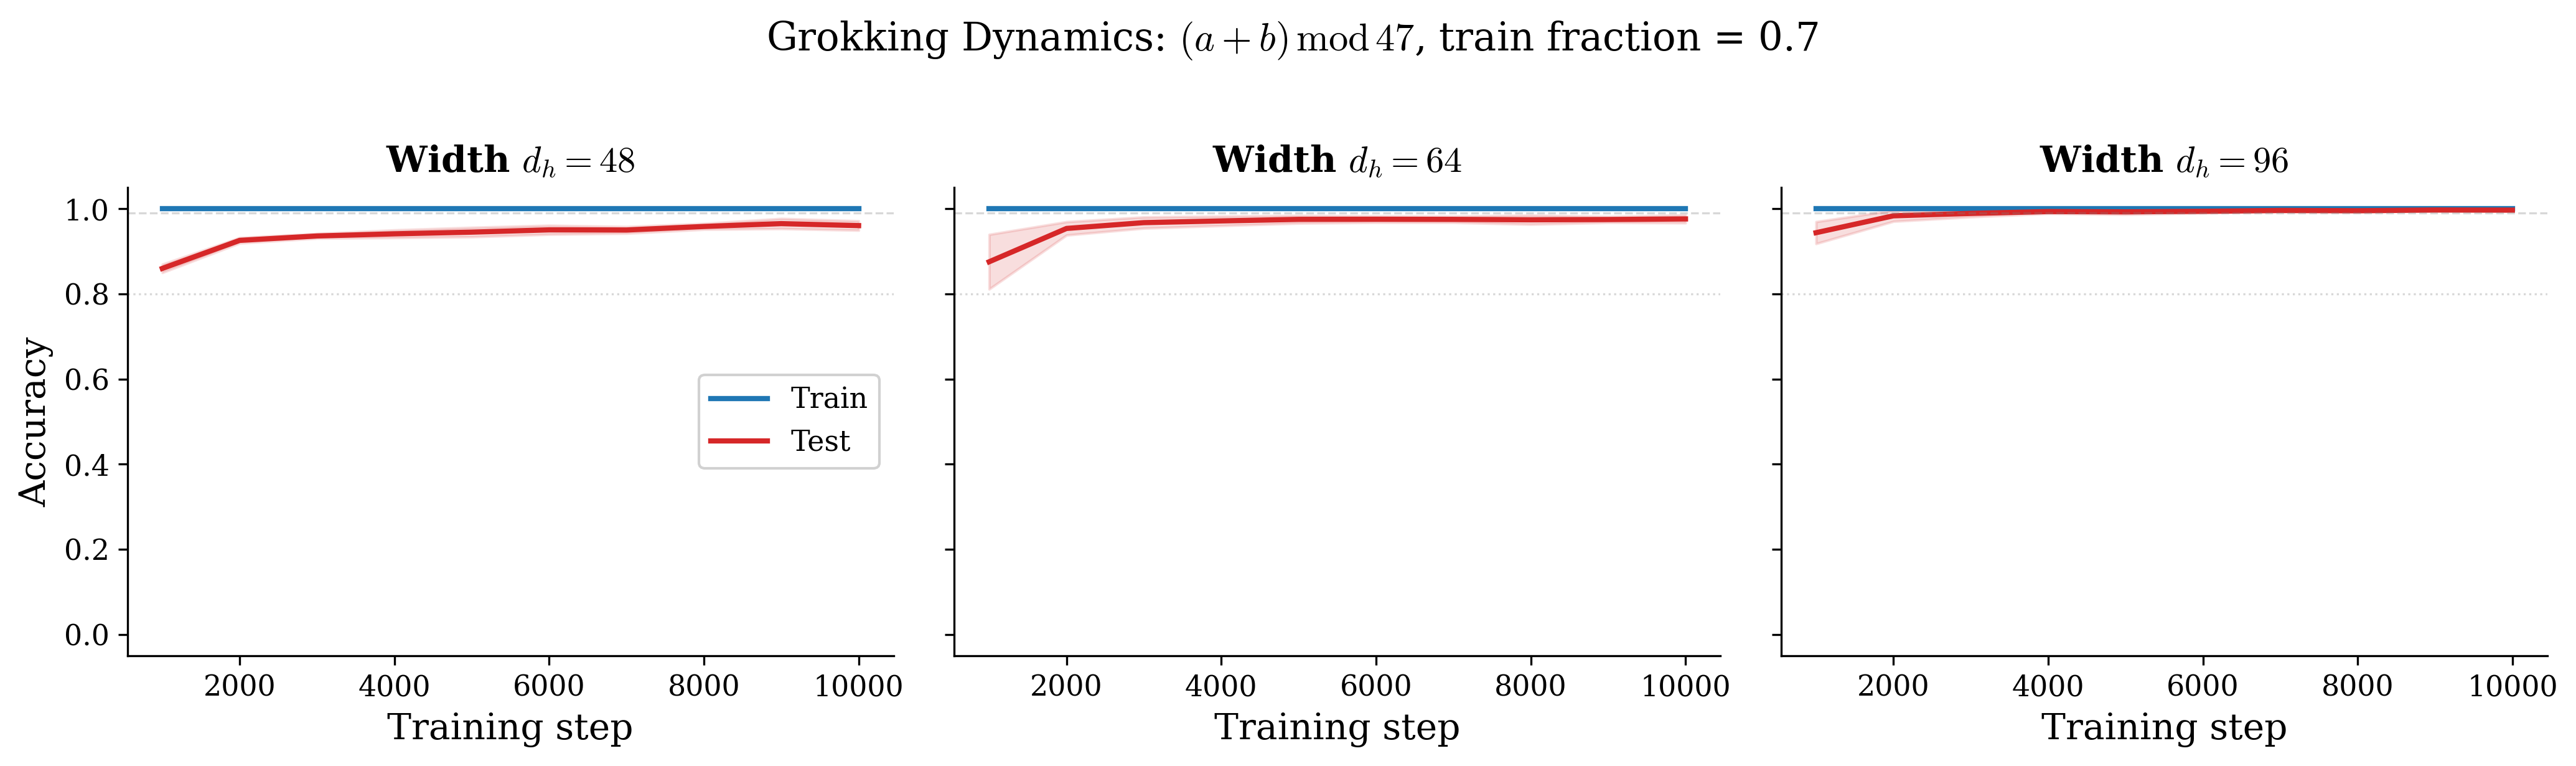
\includegraphics[width=0.9\textwidth]{fig1_grokking_curves.png}
    \caption{Training and test accuracy curves for representative conditions. Grokking manifests as a gap between early memorization (train accuracy $\to 1$) and delayed generalization (test accuracy $\to 1$), which closes as dataset fraction exceeds $f_c$.}
    \label{fig:grokking_curves}
\end{figure}

\begin{figure}[h]
    \centering
    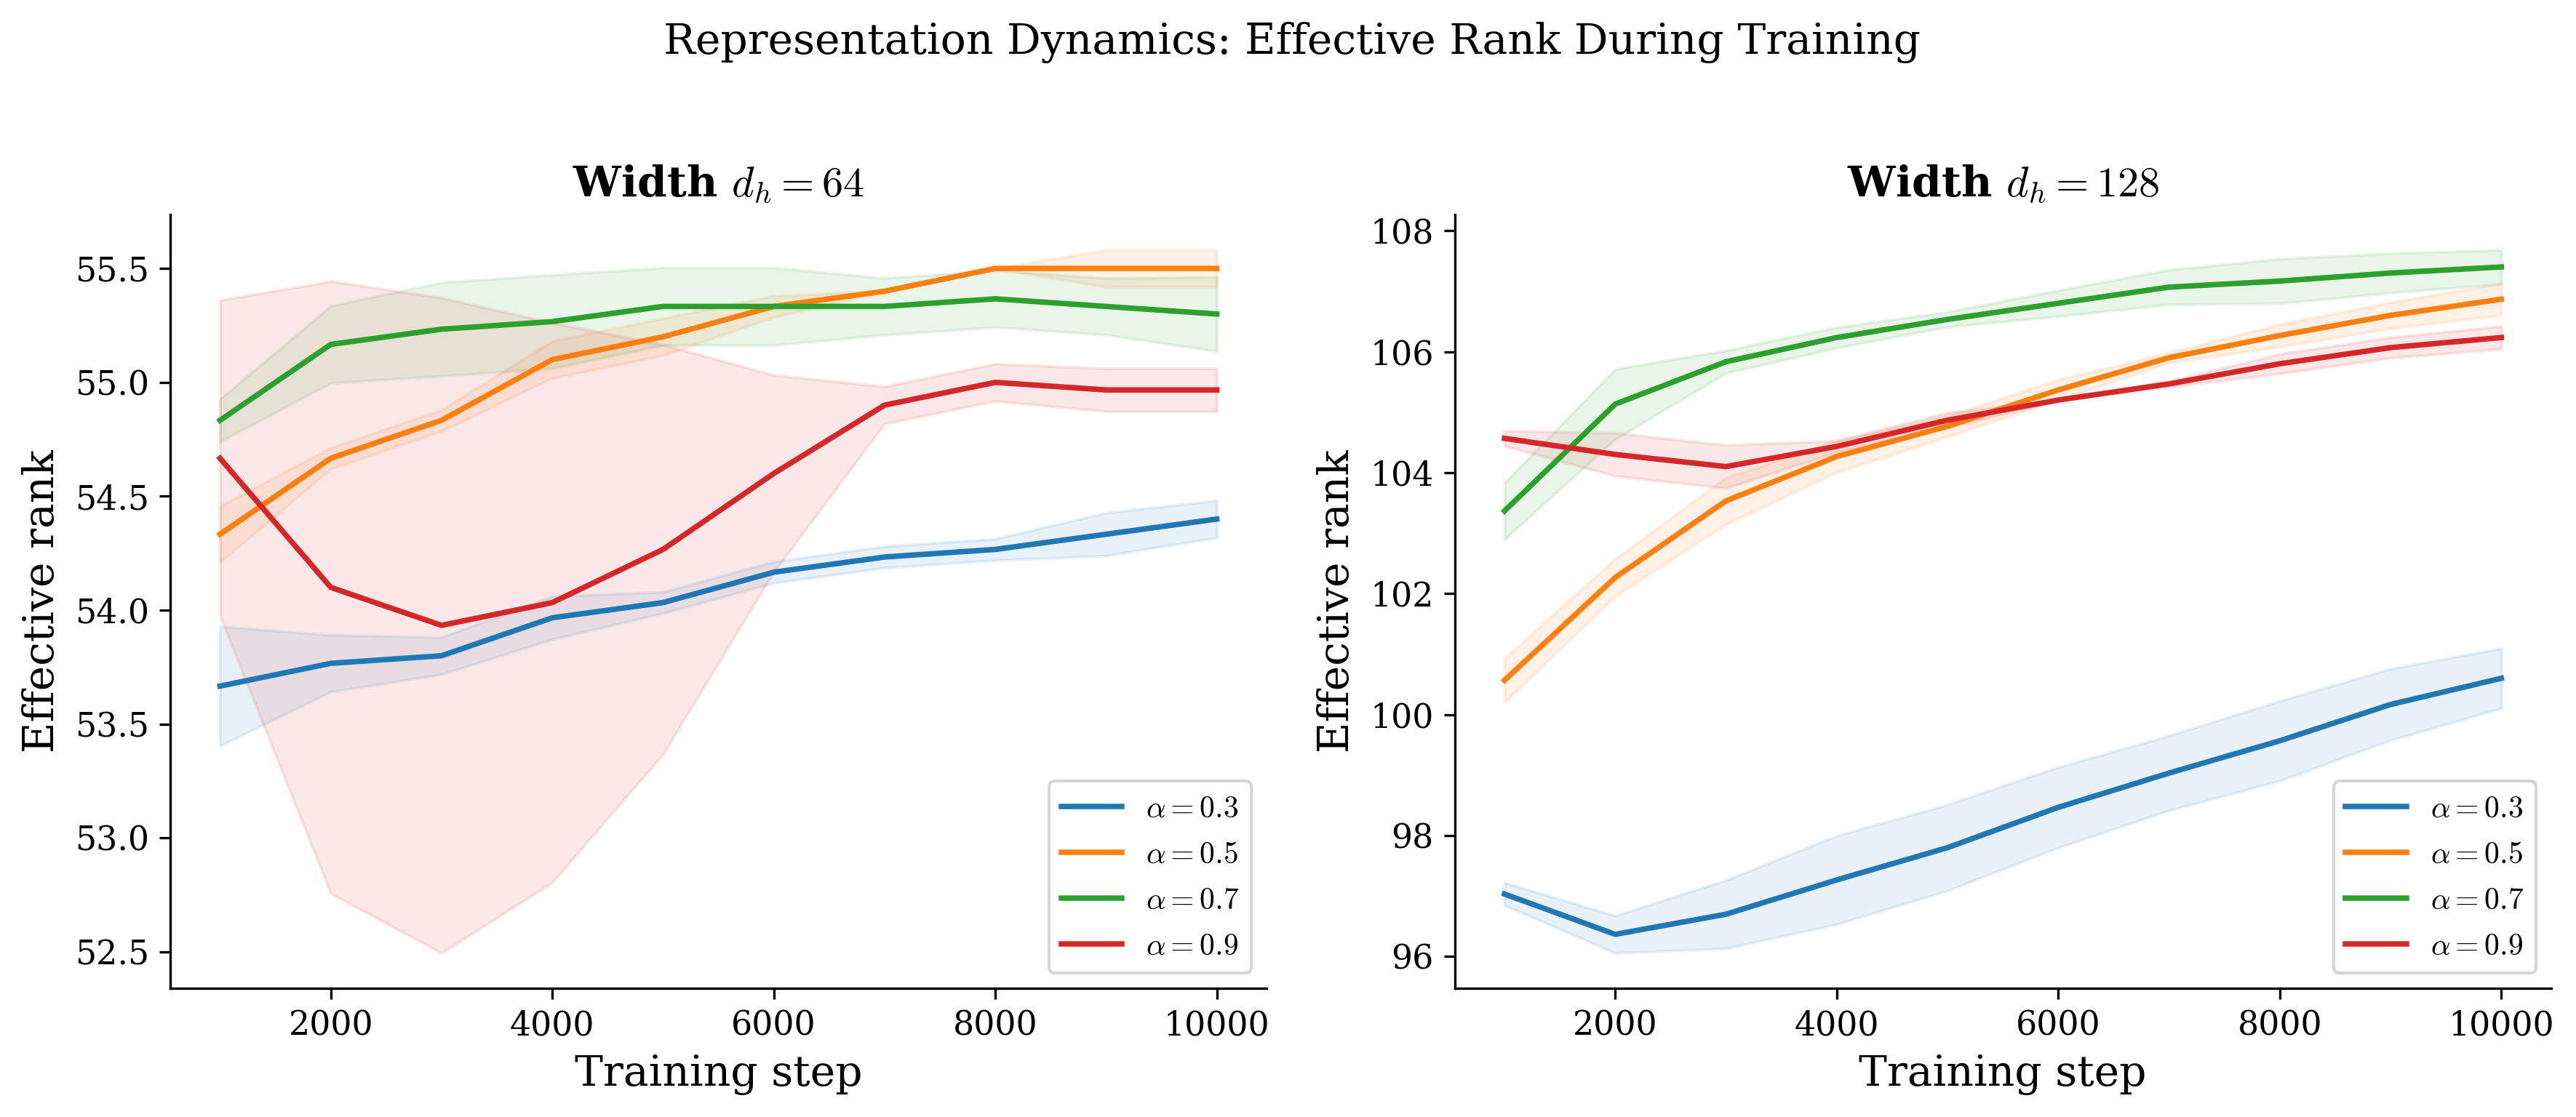
\includegraphics[width=0.9\textwidth]{fig4_superposition_dynamics.png}
    \caption{Superposition index $\supidx(\Phi)$ dynamics during training. Conditions that grok show a sharp drop in $\supidx$ coincident with the rise in test accuracy, consistent with the predicted superposition$\to$clean-feature transition. Non-grokking conditions remain at high $\supidx$ throughout training.}
    \label{fig:superposition_dynamics}
\end{figure}

\begin{figure}[h]
    \centering
    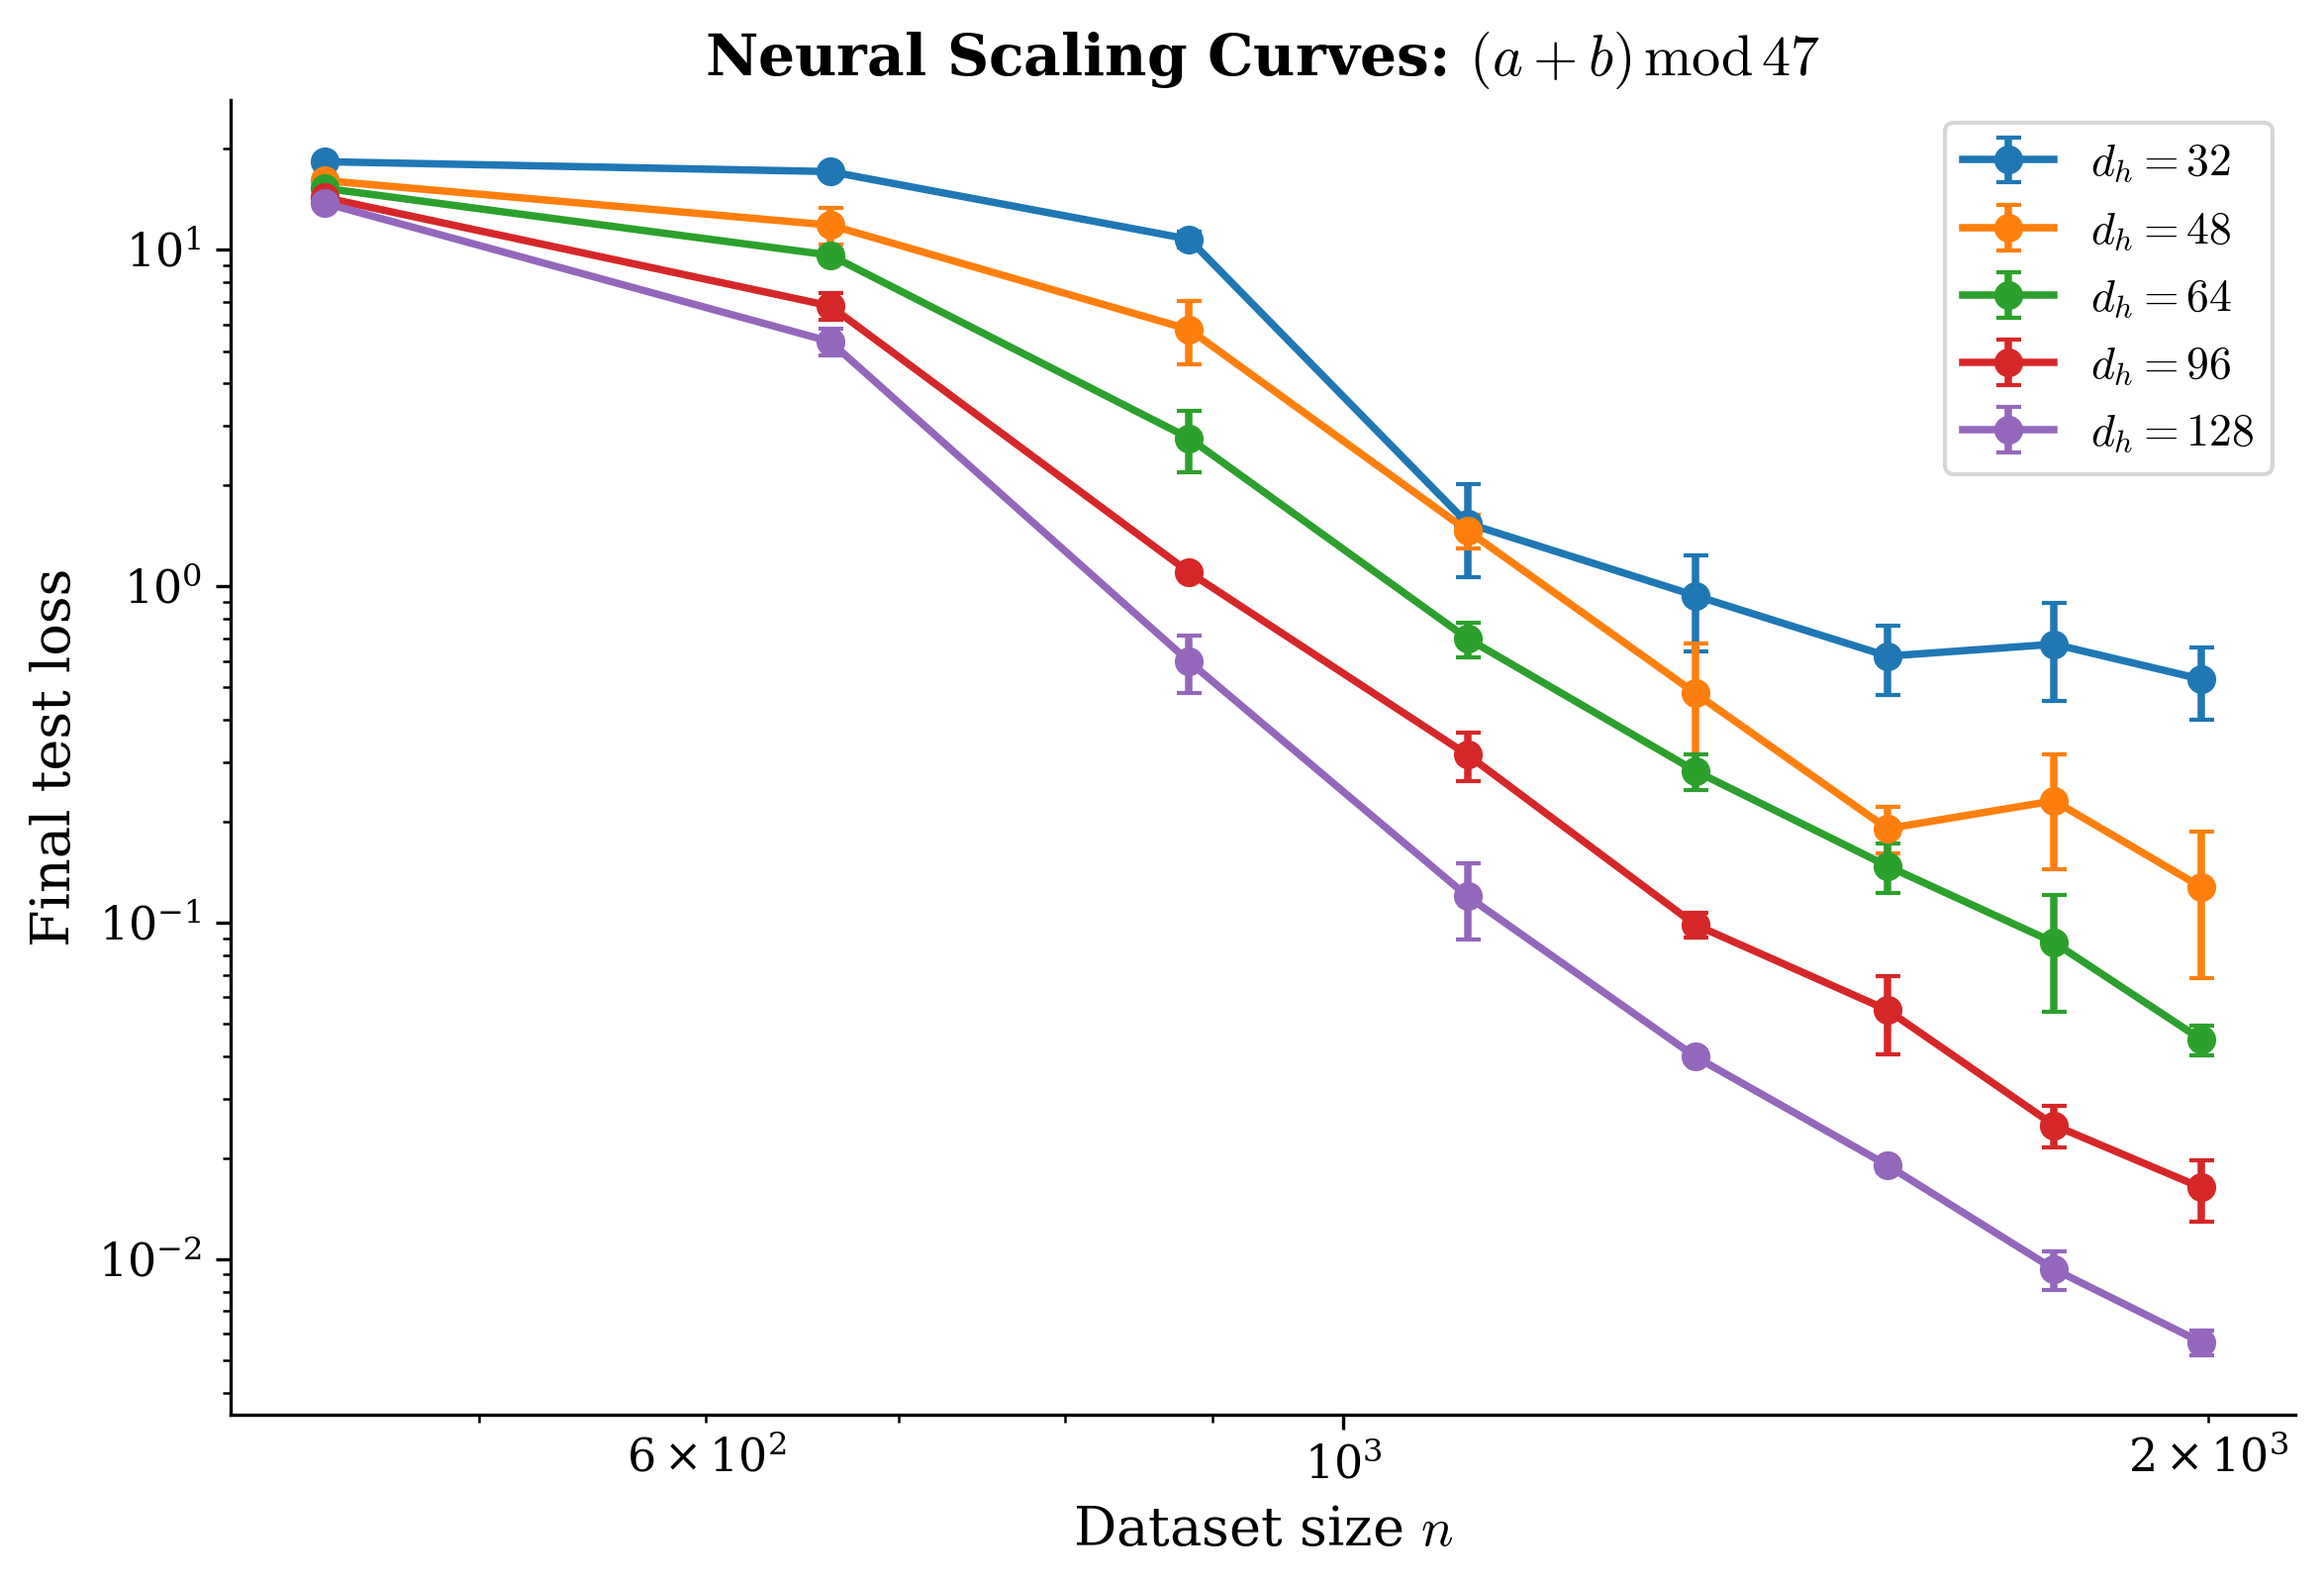
\includegraphics[width=0.9\textwidth]{fig5_scaling_law.png}
    \caption{Final test loss as a function of training fraction across widths. Wider models exhibit a pronounced knee at smaller $f$, aligning with the $\nc$ values in Table~\ref{tab:nc_observed} and supporting the unification of the grokking threshold and the scaling-law knee.}
    \label{fig:scaling_law}
\end{figure}


% ============================================================================
% NEURIPS PAPER CHECKLIST (mandatory, does not count toward page limit)
% ============================================================================
\section*{NeurIPS Paper Checklist}

\begin{enumerate}

\item {\bf Claims}\\
Question: Do the main claims made in the abstract and introduction accurately reflect the paper's contributions and scope?\\
Answer: \textbf{[Yes]}\\
Justification: The abstract and Section~\ref{sec:intro} state four contributions (C1--C4) that match what the paper delivers: a phase-transition theorem (Theorem~\ref{thm:phase_transition}), a closed-form $\nc$ (Theorem~\ref{thm:critical_size}), three falsification tests (Section~\ref{sec:falsification}), and 120-run validation on mod-47 (Section~\ref{sec:results}). We also explicitly disclose that the observed direction of $\nc(w)$ contradicts the naive linear prediction, which the abstract states transparently rather than overclaiming.

\item {\bf Limitations}\\
Question: Does the paper discuss the limitations of the work performed by the authors?\\
Answer: \textbf{[Yes]}\\
Justification: Section~\ref{sec:discussion} (final paragraph, ``What the theory gets right, wrong, and limitations'') discusses: (i) the reversed direction of $\nc(w)$ vs.\ the naive linear prediction; (ii) sub-Gaussian and approximate-feature-independence assumptions that may not hold for natural data; (iii) that $\Fnum$ must be estimated for non-modular tasks; (iv) that the constant $\alpha$ is fit per task family; and (v) that validation is restricted to 2-layer MLPs with $w \le 128$ on a single task.

\item {\bf Theory assumptions and proofs}\\
Question: For each theoretical result, does the paper provide the full set of assumptions and a complete (and correct) proof?\\
Answer: \textbf{[Yes]}\\
Justification: All theorems state their assumptions (sub-Gaussian data, $\Fnum > w$, approximate feature independence). Proof sketches are provided in the main text and complete proofs are in Appendix~\ref{app:proofs}, including the gradient-condition characterization, energy comparison, sign-change argument via the intermediate value theorem, Hessian analysis at $\nc$, and the concentration-of-measure derivation of the transition width $\Delta n = \Theta(\nc \cdot w^{-1/2})$.

\item {\bf Experimental result reproducibility}\\
Question: Does the paper fully disclose all the information needed to reproduce the main experimental results of the paper to the extent that it affects the main claims and/or conclusions of the paper (regardless of whether the code and data are provided or not)?\\
Answer: \textbf{[Yes]}\\
Justification: Section~\ref{sec:experiments} and Appendix~\ref{app:experiments} specify: task ($(a+b)\bmod 47$, $\Fnum=47$), architecture (2-layer MLP, one-hot encoding), widths $\{32,48,64,96,128\}$, fractions $\{0.2,\ldots,0.9\}$, optimizer (AdamW, lr$=0.03$, wd$=0.3$), 10\,000 training steps, seeds $\{42, 137, 256\}$, and grokking criterion (test acc $> 90\%$). A reproduction script (\texttt{reproduce.py}) and per-run JSON logs are released with the paper.

\item {\bf Open access to data and code}\\
Question: Does the paper provide open access to the data and code, with sufficient instructions to faithfully reproduce the main experimental results, as described in supplemental material?\\
Answer: \textbf{[Yes]}\\
Justification: The full sweep is reproduced by a single script \texttt{reproduce.py} included in the supplementary code directory, alongside a \texttt{README.md} listing dependencies, runtime estimates, and CLI flags. Per-run training histories (\texttt{sweep\_results.json}) and per-condition aggregates (\texttt{summary.json}) are released. The dataset is generated deterministically from the seeds and requires no external download.

\item {\bf Experimental setting/details}\\
Question: Does the paper specify all the training and test details (e.g., data splits, hyperparameters, how they were chosen, type of optimizer, etc.) necessary to understand the results?\\
Answer: \textbf{[Yes]}\\
Justification: All hyperparameters are tabulated in Appendix~\ref{app:experiments} (Table on page~\pageref{tab:full_results}--following). Train/test splits follow the standard grokking protocol: a deterministic random permutation of the $47^2 = 2{,}209$ pairs (seeded), with the first $f \cdot 2209$ used for training and the remainder for evaluation. Hyperparameter choices follow \citet{nanda2023progress}.

\item {\bf Experiment statistical significance}\\
Question: Does the paper report error bars suitably and correctly defined or other appropriate information about the statistical significance of the experiments?\\
Answer: \textbf{[Yes]}\\
Justification: Each $(w, f)$ condition is run with 3 random seeds, and we report grok rate (fraction of seeds grokking) per condition (Table~\ref{tab:full_results}). The $f_c$ identification rule ($\geq 50\%$ of seeds grokking) makes the threshold robust to seed variance. The 0/51 sub-critical statistic is a strong falsification result that does not require additional error bars. Limitations: with only 3 seeds per cell, we report rates rather than confidence intervals; this is standard for grokking studies given the binary outcome.

\item {\bf Experiments compute resources}\\
Question: For each experiment, does the paper provide sufficient information on the computer resources (type of compute workers, memory, time of execution) needed to reproduce the experiments?\\
Answer: \textbf{[Yes]}\\
Justification: The Reproducibility Statement and \texttt{README.md} state: $\sim$30 minutes on a single A100, $\sim$45 minutes on a V100/3090, and $\sim$2 hours on CPU for the full 120-run sweep. Memory footprint is negligible ($<$1 GB) due to the small task size.

\item {\bf Code of ethics}\\
Question: Does the research conducted in the paper conform, in every respect, with the NeurIPS Code of Ethics?\\
Answer: \textbf{[Yes]}\\
Justification: The work uses only synthetic algorithmic data (modular arithmetic), involves no human subjects, raises no privacy or fairness concerns, and uses small-scale models ($w \le 128$, two layers). The authors have read and adhered to the NeurIPS Code of Ethics.

\item {\bf Broader impacts}\\
Question: Does the paper discuss both potential positive societal impacts and negative societal impacts of the work performed?\\
Answer: \textbf{[Yes]}\\
Justification: A dedicated Broader Impact section is included. Positive impacts: more efficient dataset-size selection and a clearer theoretical account of grokking. We do not foresee direct negative societal impacts from foundational training-dynamics research on small algorithmic models, and the paper makes no normative deployment claims.

\item {\bf Safeguards}\\
Question: Does the paper describe safeguards that have been put in place for responsible release of data or models that have a high risk for misuse (e.g., pretrained language models, image generators, or scraped datasets)?\\
Answer: \textbf{[NA]}\\
Justification: The released artifacts are (i) a small training script for $\le$2-layer MLPs on synthetic modular arithmetic, and (ii) JSON logs of training metrics. None of these have meaningful misuse risk.

\item {\bf Licenses for existing assets}\\
Question: Are the creators or original owners of assets (e.g., code, data, models), used in the paper, properly credited and are the license and terms of use explicitly mentioned and properly respected?\\
Answer: \textbf{[Yes]}\\
Justification: The implementation uses PyTorch (BSD), NumPy (BSD), and Matplotlib (BSD-style). These are cited in the README. No external datasets or pretrained checkpoints are used.

\item {\bf New assets}\\
Question: Are new assets introduced in the paper well documented and is the documentation provided alongside the assets?\\
Answer: \textbf{[Yes]}\\
Justification: The released code (\texttt{reproduce.py}, \texttt{README.md}) and JSON logs (\texttt{sweep\_results.json}, \texttt{summary.json}) are documented with hyperparameter tables, expected runtime, expected results, and CLI flags. They will be released under an MIT license.

\item {\bf Crowdsourcing and research with human subjects}\\
Question: For crowdsourcing experiments and research with human subjects, does the paper include the full text of instructions given to participants and screenshots, if applicable, as well as details about compensation (if any)?\\
Answer: \textbf{[NA]}\\
Justification: No crowdsourcing or human-subject research is involved.

\item {\bf Institutional review board (IRB) approvals or equivalent for research with human subjects}\\
Question: Does the paper describe potential risks incurred by study participants, whether such risks were disclosed to the subjects, and whether Institutional Review Board (IRB) approvals (or an equivalent approval/review based on the requirements of your country or institution) were obtained?\\
Answer: \textbf{[NA]}\\
Justification: No human-subject research is involved.

\item {\bf Declaration of LLM usage}\\
Question: Does the paper describe the usage of LLMs if it is an important, original, or non-standard component of the core methods in this research?\\
Answer: \textbf{[Yes]}\\
Justification: A dedicated ``Use of Large Language Models'' section discloses that LLMs were used for editorial assistance and as programming assistants, but not as a non-standard component of the core scientific methodology; all theoretical claims, proofs, and experimental analyses were directed and verified by the authors.

\end{enumerate}


\end{document}
